%% ============================================================
%% Informe Técnico — Proyecto Grupal II — Big Data
%% UTEC · Facultad de Computación · Ciencias de la Computación
%% Compilar en Overleaf (pdflatex + biber no requerido)
%% ============================================================
\documentclass[12pt,a4paper]{article}

%% ── Paquetes ─────────────────────────────────────────────────
\usepackage[utf8]{inputenc}
\usepackage[T1]{fontenc}
\usepackage[spanish]{babel}
\usepackage{geometry}
\geometry{left=2.5cm, right=2.5cm, top=2.5cm, bottom=2.5cm}

\usepackage{graphicx}
\graphicspath{{img/}}
\usepackage{float}
\usepackage{caption}
\usepackage{subcaption}
\usepackage{booktabs}
\usepackage{longtable}
\usepackage{array}
\usepackage{multirow}
\usepackage{xcolor}
\usepackage{colortbl}
\usepackage{hyperref}
\usepackage{listings}
\usepackage{enumitem}
\usepackage{fancyhdr}
\usepackage{titlesec}
\usepackage{amsmath}
\usepackage{tikz}
\usetikzlibrary{shapes.geometric, arrows.meta, positioning, fit, backgrounds}

%% ── Colores Yelp + bases de datos ────────────────────────────
\definecolor{utecblue}{RGB}{196, 18, 0}      % Yelp Red principal
\definecolor{utecdark}{RGB}{130, 8, 0}       % Yelp Dark Red (títulos)
\definecolor{monggreen}{RGB}{0, 104, 56}
\definecolor{cassblue}{RGB}{30, 80, 160}
\definecolor{neo4jpurple}{RGB}{100, 50, 150}
\definecolor{airflowred}{RGB}{0, 170, 64}
\definecolor{codebg}{RGB}{255, 248, 248}     % fondo código con tinte Yelp
\definecolor{codeframe}{RGB}{196, 18, 0}

%% ── Hyperlinks ───────────────────────────────────────────────
\hypersetup{
    colorlinks=true,
    linkcolor=utecdark,
    urlcolor=utecblue,
    citecolor=utecdark,
}

%% ── Listings (código) ────────────────────────────────────────
\lstset{
    basicstyle=\ttfamily\small,
    backgroundcolor=\color{codebg},
    frame=single,
    rulecolor=\color{codeframe},
    breaklines=true,
    breakatwhitespace=true,
    tabsize=2,
    showstringspaces=false,
    xleftmargin=0.5em,
    xrightmargin=0.5em,
    numbers=none,
}
\lstdefinelanguage{CQL}{
    keywords={CREATE,TABLE,IF,NOT,EXISTS,PRIMARY,KEY,WITH,CLUSTERING,ORDER,BY,ASC,DESC,
              KEYSPACE,USE,INSERT,INTO,VALUES,SELECT,FROM,WHERE,UPDATE,SET,DELETE,ALLOW,FILTERING},
    sensitive=false,
    comment=[l]{--},
    morestring=[b]',
    morestring=[b]",
    keywordstyle=\color{utecdark}\bfseries,
    commentstyle=\color{gray}\itshape,
    stringstyle=\color{monggreen},
}
\lstdefinelanguage{Cypher}{
    keywords={MATCH,MERGE,CREATE,SET,RETURN,WITH,WHERE,ORDER,LIMIT,DELETE,DETACH,
              UNWIND,AS,ON,IN,NOT,AND,OR,DISTINCT,CONSTRAINT,INDEX,FOR,REQUIRE,IS,UNIQUE},
    sensitive=false,
    comment=[l]{//},
    morestring=[b]',
    morestring=[b]",
    keywordstyle=\color{neo4jpurple}\bfseries,
    commentstyle=\color{gray}\itshape,
    stringstyle=\color{monggreen},
}

%% ── Encabezado / pie de página ───────────────────────────────
\pagestyle{fancy}
\fancyhf{}
\fancyhead[L]{\textcolor{utecblue}{\textbf{Big Data — Proyecto Grupal II}}}
\fancyhead[R]{\textcolor{utecdark}{UTEC · 2026}}
\fancyfoot[C]{\thepage}
\renewcommand{\headrulewidth}{1pt}
\renewcommand{\headrule}{\hbox to\headwidth{\color{utecblue}\leaders\hrule height \headrulewidth\hfill}}

%% ── Formato de secciones ─────────────────────────────────────
\titleformat{\section}{\large\bfseries\color{utecdark}}{}{0em}{}[\color{utecblue}\titlerule]
\titleformat{\subsection}{\normalsize\bfseries\color{utecdark}}{}{0em}{}
\titleformat{\subsubsection}{\normalsize\itshape\color{utecdark}}{}{0em}{}

%% ══════════════════════════════════════════════════════════════
\begin{document}

%% ── Portada ──────────────────────────────────────────────────
\begin{titlepage}
\centering

%% Encabezado institucional del año
{\small\itshape ``Año de la Esperanza y el Fortalecimiento de la Democracia''}\\[1.2cm]

%% Logos: UTEC izquierda, Yelp derecha
\begin{minipage}{0.45\textwidth}
  \centering
  
\includegraphics[height=2.8cm]{utec_logo.jpg}
\end{minipage}%
\hfill
\begin{minipage}{0.45\textwidth}
  \centering
  
\includegraphics[height=2.2cm]{yelp_logo.png}
\end{minipage}

\vspace{1cm}
{\color{utecblue}\rule{\linewidth}{2pt}}
\vspace{0.5cm}

{\LARGE\bfseries\color{utecdark}
Arquitectura Multimodelo sobre el\\[0.2em]
Yelp Open Dataset}\\[0.4em]

{\color{utecblue}\rule{\linewidth}{2pt}}
\vspace{1cm}

\begin{tabular}{rl}
\textbf{Curso:}    & Big Data \\[0.2em]
\textbf{Carrera:}  & Ciencia de Datos \\[0.2em]
\textbf{Docente:}  & Lezama Benavides, Aldo Martin \\[0.2em]
\textbf{Proyecto:} & Arquitectura multimodelo con Yelp Open Dataset \\
\end{tabular}

\vspace{1.2cm}

\begin{tabular}{|c|c|}
\hline
\rowcolor[RGB]{196,18,0}
\textbf{\textcolor{white}{Integrante}} & \textbf{\textcolor{white}{Código}} \\
\hline
Quenta Solis, Jorge Eduardo      & 202310623 \\
\hline
Velo Poma, Juan David            & 202410587 \\
\hline
Cortez Rojas, Melanie Alexia     & 202210100 \\
\hline
Maguiña Aranda, Paola Mercedes   & 202120695 \\
\hline
Maquera Bobadilla, Diva Stewart  & 202310599 \\
\hline
Yangali Cáceres, Luciana         & 202310298 \\
\hline
\end{tabular}

\vfill
{\large\bfseries Lima, 06 de julio de 2026}
\end{titlepage}

\newpage
\tableofcontents
\newpage

%% ══════════════════════════════════════════════════════════════
\section{Introducción}

El presente informe documenta el desarrollo del Proyecto Grupal II del curso de Big Data
de UTEC, cuyo objetivo es diseñar e implementar un sistema de procesamiento y análisis
de datos a gran escala utilizando una arquitectura multimodelo. El proyecto toma como
fuente el \textbf{Yelp Open Dataset}, un conjunto público de reseñas, negocios, usuarios
y relaciones sociales, y hace fluir los mismos datos por tres bases de datos con propósitos
complementarios: MongoDB para documentos, Apache Cassandra para series temporales y
Apache Neo4j para el grafo social.

La orquestación del pipeline es responsabilidad de \textbf{Apache Airflow}, que ejecuta
diariamente seis etapas en secuencia: extracción, limpieza, carga en MongoDB, carga en
Cassandra, construcción del grafo en Neo4j y generación automática de nueve KPIs. Los
resultados son consultables en tiempo real a través de un \textbf{dashboard analítico}
construido con Streamlit y Plotly, que integra las tres bases de datos en una sola interfaz.

%% ══════════════════════════════════════════════════════════════
\section{Descripción del Problema}

Las plataformas de reseñas generan datos semiestructurados de alto volumen y variedad:
documentos JSON con esquemas variables por tipo de negocio, eventos con marca de tiempo
que forman series temporales, y redes sociales de usuarios con relaciones de amistad y
reseña. Un único modelo de base de datos no puede servir eficientemente los tres tipos
de acceso simultáneamente.

\textbf{Preguntas de negocio que responde el sistema:}
\begin{itemize}[noitemsep]
    \item ¿Cuántas reseñas se procesaron cada día y cómo varió ese volumen?
    \item ¿Qué categoría de negocio tiene mejor calificación en un día dado?
    \item ¿Cuál es el sentimiento promedio de los usuarios según VADER NLP?
    \item ¿Quién es el usuario más influyente en la red social y qué negocios recomienda su círculo?
    \item ¿Qué porcentaje de categorías mantiene un sentimiento positivo sostenido?
\end{itemize}

El reto técnico consiste en diseñar un pipeline reproducible y escalable que:
\begin{enumerate}[noitemsep]
    \item Simule actualizaciones incrementales diarias (un día por corrida).
    \item Cargue cada entidad en la base de datos más adecuada a su naturaleza de acceso.
    \item Genere KPIs automáticamente al final de cada corrida.
    \item Exponga todos los datos en un dashboard unificado sin duplicar lógica de negocio.
\end{enumerate}

%% ══════════════════════════════════════════════════════════════
\section{Arquitectura Propuesta}

\subsection{Diagrama general}

La arquitectura sigue el patrón \textit{extract--transform--load} (ETL) multimodelo,
orquestado por Airflow. Los datos fluyen de forma unidireccional: del almacenamiento
crudo (\texttt{data/raw/}) al área de staging limpia (\texttt{data/staging/}), y de
ahí a las tres bases de datos. El dashboard consume de las tres simultáneamente.

\begin{figure}[H]
\centering
\begin{tikzpicture}[
    every node/.style={font=\small},
    db/.style={draw, rounded corners=4pt, minimum width=2.6cm, minimum height=1cm,
               text centered, line width=1pt, align=center},
    arrow/.style={-Stealth, line width=1pt},
]

%% Nodos con coordenadas absolutas para control total del layout
\node[db, fill=gray!15]       at (0,0)    (raw)     {RAW JSON\\(Yelp Dataset)};
\node[db, fill=gray!20]       at (3.2,0)  (staging) {Staging\\JSONL limpio};

\node[db, fill=monggreen!20]  at (6.8, 1.8) (mongo) {\textcolor{monggreen}{\textbf{MongoDB}}\\documentos};
\node[db, fill=cassblue!20]   at (6.8, 0)   (cass)  {\textcolor{cassblue}{\textbf{Cassandra}}\\series temp.};
\node[db, fill=neo4jpurple!20]at (6.8,-1.8) (neo4j) {\textcolor{neo4jpurple}{\textbf{Neo4j}}\\grafo social};

\node[db, fill=green!15]      at (10.2, 0) (kpi)   {KPI Results\\(Cassandra)};
\node[db, fill=orange!20]     at (13.2, 0) (dash)  {\textbf{Dashboard}\\Streamlit};

%% Rectángulo Airflow en la capa de fondo
\begin{scope}[on background layer]
\node[draw, dashed, fill=yellow!6, rounded corners=4pt,
      fit=(staging)(mongo)(cass)(neo4j)(kpi),
      inner sep=10pt,
      label={[font=\small\bfseries]above:Apache Airflow DAG}] (airflow) {};
\end{scope}

%% Flechas
\draw[arrow] (raw)     -- (staging);
\draw[arrow] (staging) -- (mongo);
\draw[arrow] (staging) -- (cass);
\draw[arrow] (staging) -- (neo4j);
\draw[arrow] (mongo)   -| (kpi);
\draw[arrow] (cass)    -- (kpi) node[midway, above, font=\tiny]{generate\_kpis};
\draw[arrow] (neo4j)   -| (kpi);
\draw[arrow] (mongo.east)  to[out=0,in=150] (dash.north west);
\draw[arrow] (kpi)     -- (dash);
\draw[arrow] (neo4j.east) to[out=0,in=210] (dash.south west);

\end{tikzpicture}
\caption{Arquitectura multimodelo del sistema. Los datos fluyen en una sola dirección: raw $\to$ staging $\to$ BDs $\to$ KPIs $\to$ dashboard.}
\end{figure}

\subsection{Justificación técnica de cada base de datos}

\begin{longtable}{>{\bfseries}p{2.8cm} p{5cm} p{6cm}}
\toprule
Base de datos & Entidad almacenada & Justificación \\
\midrule
\textcolor{monggreen}{MongoDB} &
Businesses, Reviews, Users, Tips &
El campo \texttt{attributes} de los negocios tiene esquema variable por tipo (un restaurante tiene \texttt{NoiseLevel}, una lavandería no). MongoDB permite esquemas flexibles y consultas sobre documentos anidados sin necesidad de definir una tabla rígida. \\[0.4em]

\textcolor{cassblue}{Cassandra} &
Reviews por negocio y fecha, conteos diarios, stats por categoría, KPIs &
Las reseñas son eventos con marca de tiempo: escrituras masivas y consultas ``dame todas las reseñas de este negocio entre X e Y'' son exactamente el caso de uso de Cassandra. El modelo \textit{query-first} permite diseñar la partición exactamente para esa consulta. \\[0.4em]

\textcolor{neo4jpurple}{Neo4j} &
Usuarios, Negocios, Categorías, Ciudades; relaciones FRIEND, REVIEWED, IN\_CATEGORY, LOCATED\_IN &
El campo \texttt{friends} de cada usuario crea una red social real. Las consultas de influencia (``¿qué negocios visita el círculo del usuario con más amigos?'') requieren traversals de grafo que en SQL serían JOINs recursivos; Neo4j los ejecuta de forma nativa. \\
\bottomrule
\end{longtable}

%% ══════════════════════════════════════════════════════════════
\section{Descripción del Dataset}

\subsection{Fuente y licencia}

El \textbf{Yelp Open Dataset} es un conjunto de datos público de uso académico disponible
en \url{https://business.yelp.com/data/resources/open-dataset/}. El dataset contiene
información de negocios, usuarios, reseñas, tips y check-ins de múltiples ciudades de
Estados Unidos y Canadá.

\subsection{Filtro aplicado}

Para mantener el proyecto manejable y geográficamente cohesivo, se filtró a
\textbf{Philadelphia, Pennsylvania (PA)}, lo que resultó en el subconjunto descrito
en la Tabla~\ref{tab:dataset}.

\begin{table}[H]
\centering
\caption{Volumen del dataset filtrado a Philadelphia, PA}
\label{tab:dataset}
\begin{tabular}{lrrl}
\toprule
\textbf{Entidad} & \textbf{Registros} & \textbf{Tamaño aprox.} & \textbf{Destino} \\
\midrule
Businesses & 14,567 & — & MongoDB + Neo4j \\
Reviews    & 200,000 & — & MongoDB + Cassandra \\
Users      & 98,138 & — & MongoDB + Neo4j \\
Tips       & 115,910 & — & MongoDB \\
Check-ins  & — & — & Cassandra \\
\midrule
\textbf{Total reviews (fechas)} & 5,572 días & 2005-06-27 a 2022-01-19 & — \\
\bottomrule
\end{tabular}
\end{table}

\subsection{Estructura de los archivos fuente}

Los archivos originales de Yelp son JSON Lines (un objeto JSON por línea):

\begin{table}[H]
\centering
\caption{Estructura de los archivos JSON del dataset}
\begin{tabular}{p{2.5cm} p{6.5cm} p{5cm}}
\toprule
\textbf{Archivo} & \textbf{Campos clave} & \textbf{Característica especial} \\
\midrule
\texttt{business.json} & \texttt{business\_id, name, city, stars, categories, attributes} & \texttt{attributes} es anidado y variable \\
\texttt{review.json} & \texttt{review\_id, user\_id, business\_id, stars, text, date} & \texttt{text} enriquecido con VADER NLP \\
\texttt{user.json} & \texttt{user\_id, name, review\_count, friends, fans} & \texttt{friends} es lista de user\_ids \\
\texttt{tip.json} & \texttt{user\_id, business\_id, text, date, compliment\_count} & Comentarios cortos \\
\texttt{checkin.json} & \texttt{business\_id, date} & Lista de timestamps separados por coma \\
\bottomrule
\end{tabular}
\end{table}

\subsection{Enriquecimiento aplicado}

Durante la etapa de limpieza se añade el campo \texttt{sentiment} a cada reseña usando
el modelo \textbf{VADER} (\textit{Valence Aware Dictionary and sEntiment Reasoner}),
que devuelve un score compuesto entre $-1$ (muy negativo) y $+1$ (muy positivo)
sin necesidad de entrenamiento previo. Este campo alimenta los KPIs 6, 7, 8 y 9.

%% ══════════════════════════════════════════════════════════════
\section{Modelo de Datos de MongoDB}

\subsection{Base de datos y colecciones}

La base de datos se llama \texttt{yelp} y contiene cuatro colecciones. Todos los
documentos usan el \texttt{\_id} nativo de MongoDB igualado al identificador único
del objeto Yelp (estrategia upsert idempotente).

\begin{longtable}{>{\ttfamily}p{2.5cm} p{4.5cm} p{6cm}}
\toprule
\normalfont\textbf{Colección} & \textbf{Campos principales} & \textbf{Notas} \\
\midrule
businesses &
\texttt{\_id} (=business\_id), name, address, city, state, stars, review\_count, categories (array), attributes (subdocumento), hours (subdocumento) &
\texttt{attributes} contiene propiedades como \texttt{RestaurantsDelivery}, \texttt{WiFi}, \texttt{NoiseLevel} que varían por tipo de negocio. Aprovecha el esquema flexible de MongoDB. \\[0.5em]

reviews &
\texttt{\_id} (=review\_id), user\_id, business\_id, stars, text, date, useful, funny, cool, sentiment (float) &
\texttt{sentiment} es calculado en la etapa de limpieza mediante VADER. Campo \texttt{date} indexado para consultas temporales. \\[0.5em]

users &
\texttt{\_id} (=user\_id), name, review\_count, yelping\_since, fans, average\_stars, friends (array) &
\texttt{friends} puede contener miles de user\_ids. En MongoDB se almacena como lista; en Neo4j se convierte en aristas FRIEND. \\[0.5em]

tips &
user\_id, business\_id, text, date, compliment\_count &
No tiene \texttt{\_id} propio de Yelp; se usa índice compuesto \{user\_id, business\_id, date\} como clave de upsert. \\
\bottomrule
\end{longtable}

\subsection{Índices}

Se crean los siguientes índices para optimizar las consultas del dashboard:

\begin{lstlisting}[language={}]
-- businesses
db.businesses.createIndex({ city: 1 })
db.businesses.createIndex({ stars: -1 })
db.businesses.createIndex({ categories: 1 })   -- multikey

-- reviews
db.reviews.createIndex({ business_id: 1, date: 1 })
db.reviews.createIndex({ stars: -1 })

-- users
db.users.createIndex({ review_count: -1 })
\end{lstlisting}

\subsection{Operaciones CRUD}

\begin{longtable}{>{\bfseries}p{2.5cm} >{\ttfamily\small\raggedright\arraybackslash}p{6.5cm} >{\raggedright\arraybackslash}p{5cm}}
\toprule
\normalfont\textbf{Operación} & \normalfont\textbf{Ejemplo} & \normalfont\textbf{Descripción} \\
\midrule
Create &
db.businesses.insert\_one(\{...\}) &
Insertar nuevo negocio manualmente. \\[0.3em]

Read &
db.reviews.find(\{business\_id: "X"\}) &
Buscar todas las reseñas de un negocio. \\[0.3em]

Update &
db.businesses.update\_one( \{\_id: "X"\}, \{\$set: \{stars: 4.5\}\} ) &
Actualizar el rating de un negocio. \\[0.3em]

Delete &
db.reviews.delete\_one(\{\_id: "review\_id"\}) &
Eliminar una reseña específica. \\
\bottomrule
\end{longtable}

%% ══════════════════════════════════════════════════════════════
\section{Modelo de Datos de Cassandra}

\subsection{Keyspace}

\begin{lstlisting}[language=CQL]
CREATE KEYSPACE IF NOT EXISTS yelp_analytics
  WITH replication = {'class': 'SimpleStrategy', 'replication_factor': 1};
\end{lstlisting}

\subsection{Tablas}

El diseño sigue el principio \textit{query-first} de Cassandra: cada tabla está
optimizada para una consulta específica del pipeline o del dashboard.

\begin{longtable}{>{\ttfamily\small}p{4.8cm} p{4cm} p{5cm}}
\toprule
\normalfont\textbf{Tabla} & \normalfont\textbf{Partition / Clustering Key} & \normalfont\textbf{Consulta objetivo} \\
\midrule

reviews\_by\_business\_date &
PK: \texttt{(business\_id)}, CK: \texttt{review\_date DESC, review\_id} &
``Dame todas las reseñas del negocio X ordenadas por fecha''. \\[0.4em]

daily\_review\_counts &
PK: \texttt{(year\_month)}, CK: \texttt{review\_date ASC} &
``¿Cuántas reseñas hubo cada día del mes?'' Partición por año-mes evita particiones infinitas. \\[0.4em]

category\_daily\_stats &
PK: \texttt{(category)}, CK: \texttt{stat\_date ASC} &
``Evolución temporal del rating y sentimiento de la categoría X.'' \\[0.4em]

checkins\_by\_business &
PK: \texttt{(business\_id)}, CK: \texttt{checkin\_ts DESC} &
``Check-ins recientes del negocio X.'' \\[0.4em]

kpi\_results &
PK: \texttt{(kpi\_name)}, CK: \texttt{kpi\_date DESC} &
``Valor del KPI Y para todas las fechas disponibles.'' \\
\bottomrule
\end{longtable}

\subsubsection{DDL completo de las tablas principales}

\begin{lstlisting}[language=CQL]
CREATE TABLE IF NOT EXISTS reviews_by_business_date (
  business_id  text,
  review_date  date,
  review_id    text,
  stars        float,
  user_id      text,
  PRIMARY KEY ((business_id), review_date, review_id)
) WITH CLUSTERING ORDER BY (review_date DESC);

CREATE TABLE IF NOT EXISTS daily_review_counts (
  year_month   text,
  review_date  date,
  total        int,
  PRIMARY KEY ((year_month), review_date)
) WITH CLUSTERING ORDER BY (review_date ASC);

CREATE TABLE IF NOT EXISTS category_daily_stats (
  category      text,
  stat_date     date,
  review_count  int,
  avg_stars     float,
  avg_sentiment float,
  PRIMARY KEY ((category), stat_date)
) WITH CLUSTERING ORDER BY (stat_date ASC);

CREATE TABLE IF NOT EXISTS kpi_results (
  kpi_name  text,
  kpi_date  date,
  value     double,
  detail    text,
  PRIMARY KEY ((kpi_name), kpi_date)
) WITH CLUSTERING ORDER BY (kpi_date DESC);
\end{lstlisting}

\subsection{Operaciones CRUD}

\begin{longtable}{>{\bfseries}p{2.5cm} >{\ttfamily\small\raggedright\arraybackslash}p{7cm} >{\raggedright\arraybackslash}p{4cm}}
\toprule
\normalfont\textbf{Operación} & \normalfont\textbf{Ejemplo CQL} & \normalfont\textbf{Descripción} \\
\midrule
Insert &
INSERT INTO kpi\_results (kpi\_name, kpi\_date, value, detail) VALUES ('reviews\_per\_day', '2022-01-19', 24.0, 'n reseñas'); &
Insertar un KPI calculado. \\[0.3em]

Query &
SELECT * FROM daily\_review\_counts WHERE year\_month='2022-01'; &
Consultar todos los días de enero 2022. \\[0.3em]

Update &
UPDATE category\_daily\_stats SET avg\_stars=4.2 WHERE category='Restaurants' AND stat\_date='2022-01-19'; &
Actualizar el rating de una categoría. \\[0.3em]

Delete &
DELETE FROM kpi\_results WHERE kpi\_name='reviews\_per\_day' AND kpi\_date='2026-07-03'; &
Eliminar un KPI de fecha incorrecta. \\
\bottomrule
\end{longtable}

%% ══════════════════════════════════════════════════════════════
\section{Modelo de Grafo en Neo4j}

\subsection{Nodos y propiedades}

\begin{table}[H]
\centering
\caption{Nodos del grafo Neo4j}
\begin{tabular}{>{\ttfamily}p{1.8cm} p{5.5cm} p{6.5cm}}
\toprule
\normalfont\textbf{Etiqueta} & \textbf{Propiedades} & \textbf{Descripción} \\
\midrule
\texttt{User}     & user\_id, name, review\_count, fans, average\_stars & Usuario de Yelp. 98,138 nodos. \\
\texttt{Business} & business\_id, name, city, stars, review\_count      & Negocio de Philadelphia. 14,567 nodos. \\
\texttt{Category} & name                                                 & Categoría de negocio (ej. ``Restaurants''). \\
\texttt{City}     & name, state                                         & Ciudad para consultas geográficas. \\
\bottomrule
\end{tabular}
\end{table}

\subsection{Relaciones}

\begin{table}[H]
\centering
\caption{Relaciones del grafo Neo4j}
\begin{tabular}{llp{7cm}}
\toprule
\textbf{Relación} & \textbf{Dirección} & \textbf{Descripción} \\
\midrule
\texttt{FRIEND}      & (User)$\to$(User)     & Amistad de Yelp. $\sim$530,000 aristas. \\
\texttt{REVIEWED}    & (User)$\to$(Business) & Un usuario escribió una reseña sobre un negocio. $\sim$200,000 aristas. \\
\texttt{IN\_CATEGORY}& (Business)$\to$(Category) & El negocio pertenece a una categoría. \\
\texttt{LOCATED\_IN} & (Business)$\to$(City)  & El negocio está ubicado en la ciudad. \\
\bottomrule
\end{tabular}
\end{table}

\subsection{Diagrama del grafo}

\begin{figure}[H]
\centering
\begin{tikzpicture}[
    nodo/.style={draw, circle, minimum size=1.5cm, font=\small\bfseries,
                 line width=1pt, align=center},
    rel/.style={-Stealth, line width=1pt, font=\scriptsize},
]
%% Layout: Users arriba, Business centro-izquierda,
%%         Category centro-derecha, City abajo-derecha
\node[nodo, fill=blue!25]   at (0, 0)     (u1)   {User};
\node[nodo, fill=blue!25]   at (5, 0)     (u2)   {User};
\node[nodo, fill=green!25]  at (2, -3)    (b)    {Business};
\node[nodo, fill=orange!25] at (6, -2.2)  (cat)  {Category};
\node[nodo, fill=gray!25]   at (6, -4.5)  (city) {City};

%% Relaciones
\draw[rel, bend left=20] (u1) to node[above]{FRIEND} (u2);
\draw[rel] (u1) -- node[left]{REVIEWED} (b);
\draw[rel] (u2) -- node[right, pos=0.35]{REVIEWED} (b);
\draw[rel] (b)  -- node[above, sloped]{IN\_CATEGORY} (cat);
\draw[rel] (b)  -- node[below, sloped]{LOCATED\_IN}  (city);
\end{tikzpicture}
\caption{Modelo de grafo en Neo4j: cuatro tipos de nodo y cuatro tipos de relación.}
\end{figure}

\subsection{Constraints e índices}

\begin{lstlisting}[language=Cypher]
CREATE CONSTRAINT user_id IF NOT EXISTS
  FOR (u:User) REQUIRE u.user_id IS UNIQUE;

CREATE CONSTRAINT biz_id IF NOT EXISTS
  FOR (b:Business) REQUIRE b.business_id IS UNIQUE;

CREATE CONSTRAINT cat_name IF NOT EXISTS
  FOR (c:Category) REQUIRE c.name IS UNIQUE;

CREATE INDEX user_name IF NOT EXISTS FOR (u:User) ON (u.name);
CREATE INDEX biz_stars  IF NOT EXISTS FOR (b:Business) ON (b.stars);
\end{lstlisting}

\subsection{Operaciones CRUD}

\begin{longtable}{>{\bfseries}p{2.2cm} p{5.2cm} p{5.8cm}}
\toprule
Operación & Cypher & Descripción \\
\midrule
Create nodo &
\texttt{CREATE (u:User \{user\_id: 'X', name: 'Ana'\})} &
Crear un nuevo usuario en el grafo. \\

Create relación &
\texttt{MATCH (u:User \{user\_id:'A'\}), (b:Business \{business\_id:'B'\}) CREATE (u)-[:REVIEWED]->(b)} &
Registrar que el usuario A reseñó el negocio B. \\

Read &
\texttt{MATCH (u:User)-[:FRIEND]->(f) RETURN u.name, count(f) ORDER BY count(f) DESC LIMIT 5} &
Top 5 usuarios con más amigos. \\

Update &
\texttt{MATCH (b:Business \{business\_id:'X'\}) SET b.stars = 4.5} &
Actualizar el rating de un negocio. \\

Delete &
\texttt{MATCH (u:User \{user\_id:'X'\})-[r:FRIEND]->() DELETE r} &
Eliminar todas las amistades de un usuario. \\
\bottomrule
\end{longtable}

%% ══════════════════════════════════════════════════════════════
\section{Explicación del DAG de Airflow}

\subsection{Configuración del DAG}

\begin{lstlisting}[language=Python]
dag_id    = "yelp_pipeline"
schedule  = "@daily"
start_date = datetime(2019, 1, 26)
catchup   = False   # solo corre para la fecha actual
max_active_runs = 1
\end{lstlisting}

Con \texttt{catchup=False}, el DAG no intenta ponerse al día con los días pasados al ser
activado. Para procesar datos históricos se utiliza el script \texttt{bulk\_ingest.py}
(carga masiva de 200,000 reseñas) y \texttt{backfill\_kpis.py} (5,574 fechas en $\sim$4.5 minutos).

\subsection{Flujo de tareas}

\[
\text{extract} \;\to\; \text{validate\_clean} \;\to\;
\begin{cases} \text{load\_mongo} \\ \text{transform\_load\_cassandra} \\ \text{build\_load\_neo4j} \end{cases}
\;\to\; \text{generate\_kpis}
\]

Las tres cargas corren en \textbf{paralelo} tras la limpieza, ya que los tres loaders
leen independientemente de \texttt{data/staging/} sin depender entre sí.
Esto reduce el tiempo total del pipeline y refleja correctamente que MongoDB, Cassandra
y Neo4j son sistemas independientes que consumen el mismo staging.

\subsection{Descripción de cada etapa}

\begin{longtable}{>{\bfseries\ttfamily\small}p{5cm} p{2.5cm} p{6.5cm}}
\toprule
\normalfont\textbf{Task ID} & \textbf{Duración aprox.} & \textbf{Descripción} \\
\midrule

extract &
$< 5$s &
Verifica que existen los archivos raw (o \texttt{\_sample} / \texttt{\_demo}). Lanza \texttt{FileNotFoundError} si falta alguno, forzando un retry. \\[0.3em]

validate\_clean &
$10$–$30$s &
Llama a \texttt{clean.build\_staging\_for\_date(ds)}: filtra Philadelphia PA, valida campos obligatorios, aplica VADER al texto de las reseñas y escribe JSONL particionado por fecha en \texttt{data/staging/}. \\[0.3em]

load\_mongo &
$5$–$15$s &
Carga businesses, reviews del día, users y tips en MongoDB usando \texttt{bulk\_write} con upsert. Idempotente: re-ejecutar no duplica datos. \\[0.3em]

transform\_load\_cassandra &
$5$–$20$s &
Carga \texttt{reviews\_by\_business\_date}, actualiza \texttt{daily\_review\_counts} y \texttt{category\_daily\_stats} para la fecha \texttt{ds}. \\[0.3em]

build\_load\_neo4j &
$10$–$30$s &
Hace MERGE de nodos User y Business, construye aristas REVIEWED y FRIEND con Cypher usando batches de 500 nodos. \\[0.3em]

generate\_kpis &
$2$–$5$s &
Ejecuta \texttt{compute\_kpis.run(ds)}: calcula los 9 KPIs dinámicos y los persiste en la tabla \texttt{kpi\_results} de Cassandra. \\
\bottomrule
\end{longtable}

\begin{figure}[H]
\centering
% SCREENSHOT: captura del DAG en la vista "Grid" de Airflow UI (localhost:8080)
% con todas las tareas en verde (estado success)
\fbox{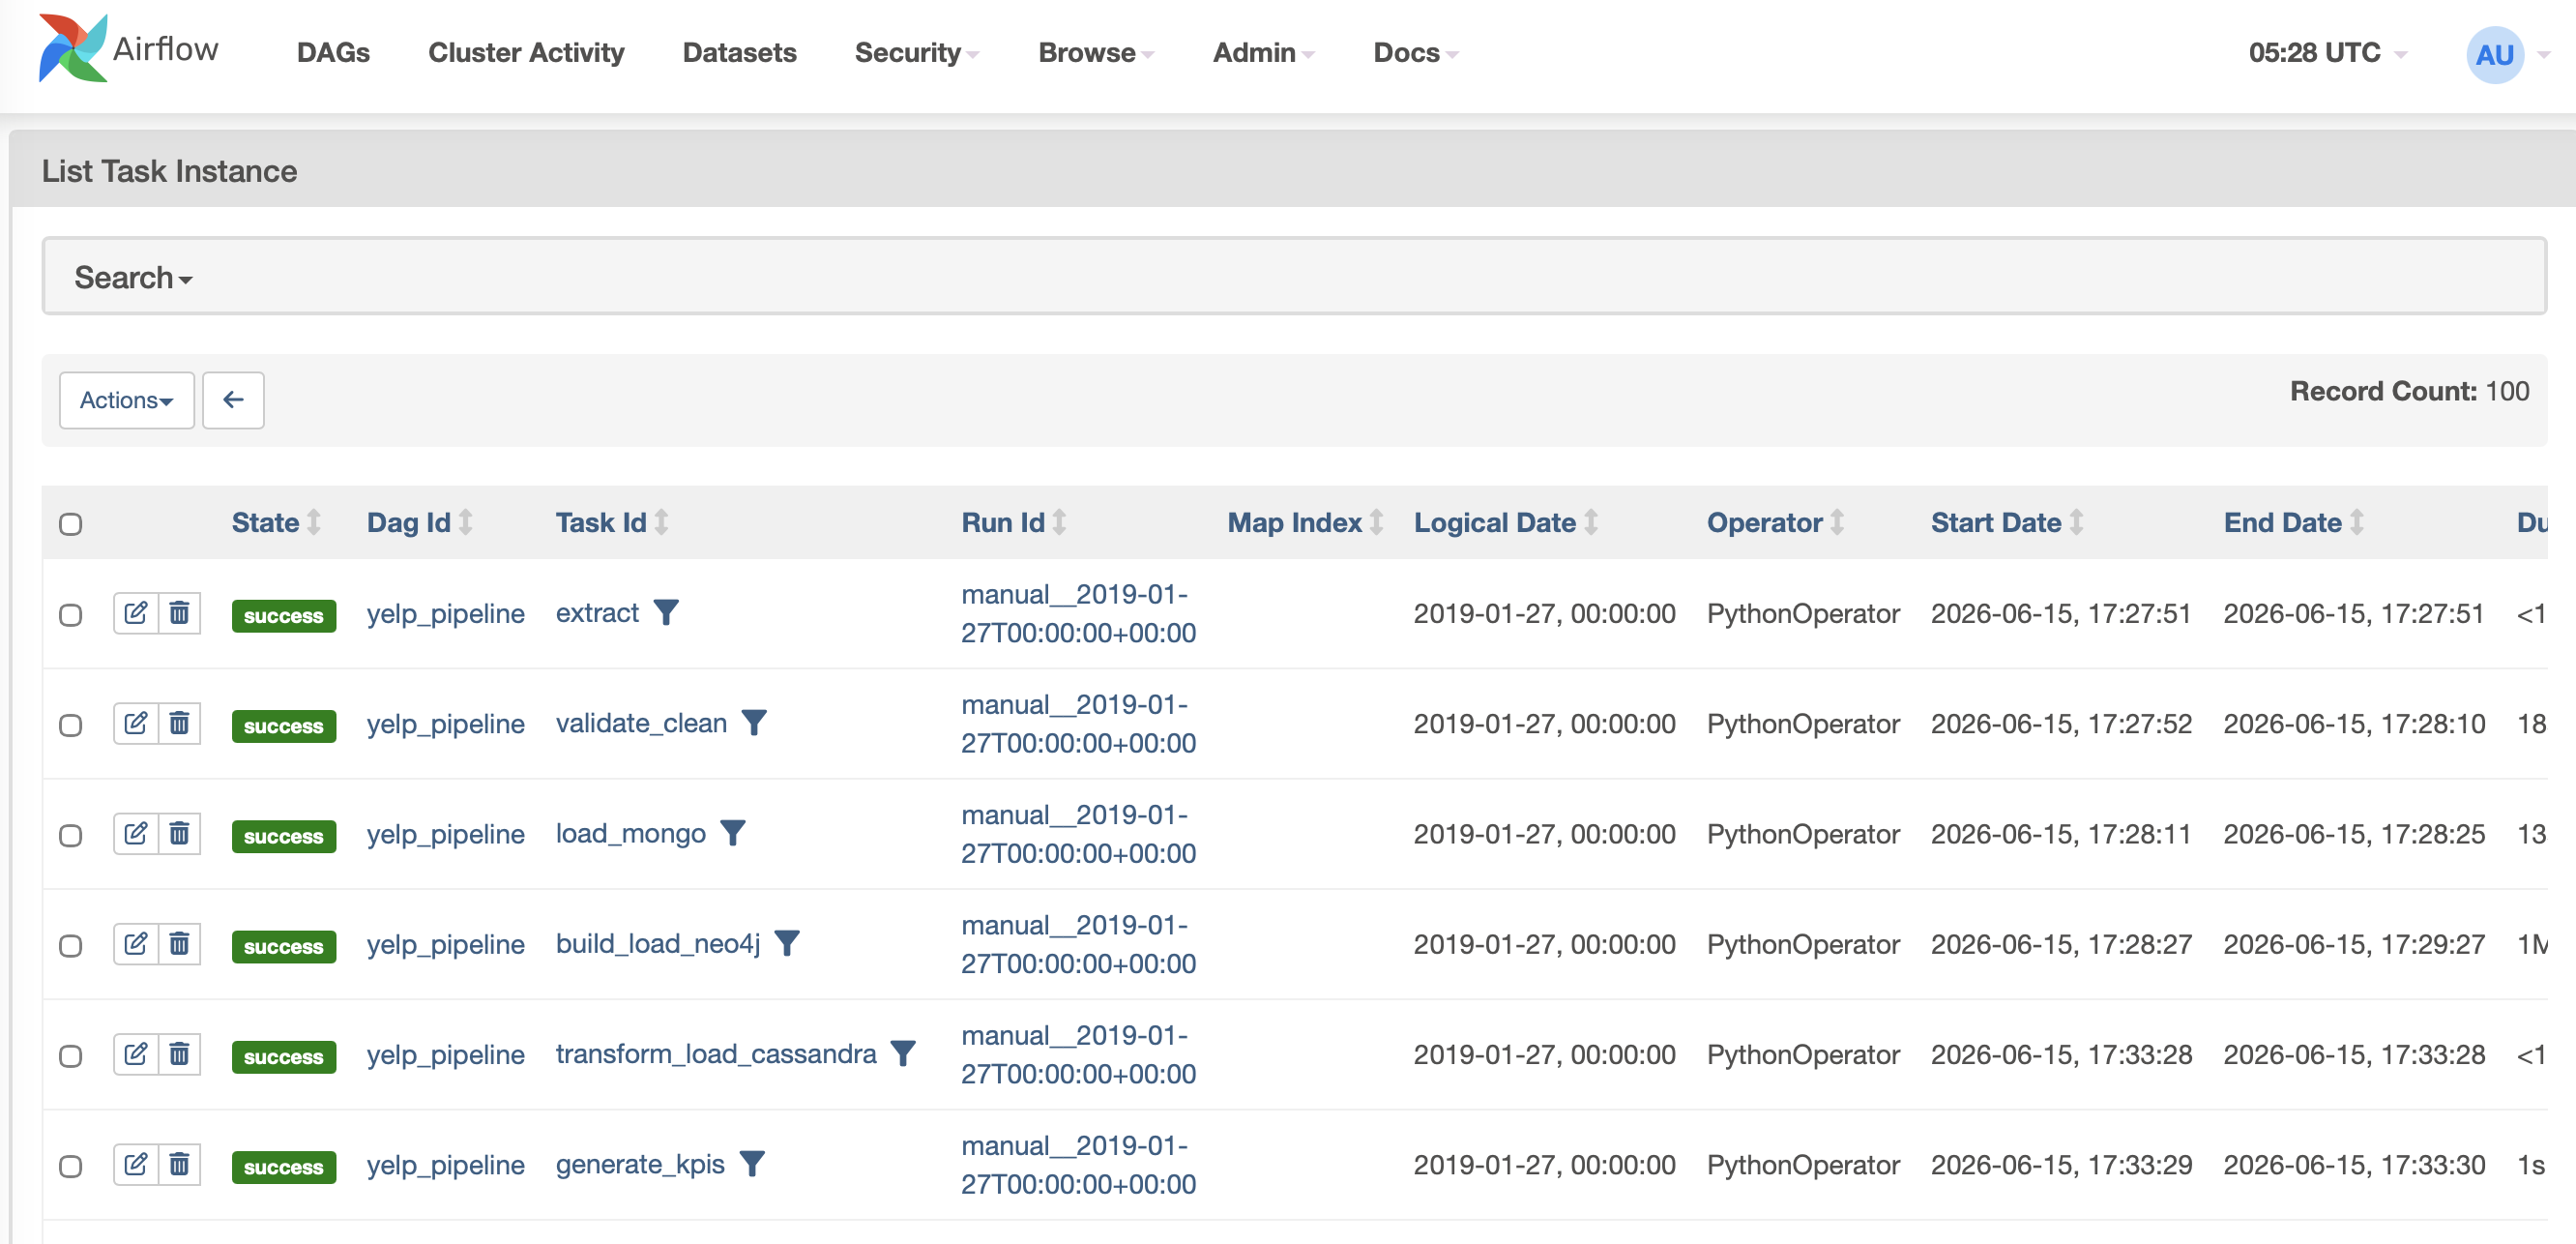
\includegraphics[width=0.9\textwidth]{img/airflow_dag_grid.png}}
\caption{Vista Grid del DAG \texttt{yelp\_pipeline} en Airflow UI mostrando una ejecución exitosa de las 6 etapas.}
\label{fig:airflow_grid}
\end{figure}

\begin{figure}[H]
\centering
% SCREENSHOT: captura de la vista "Graph" del DAG mostrando el flujo de tareas
\fbox{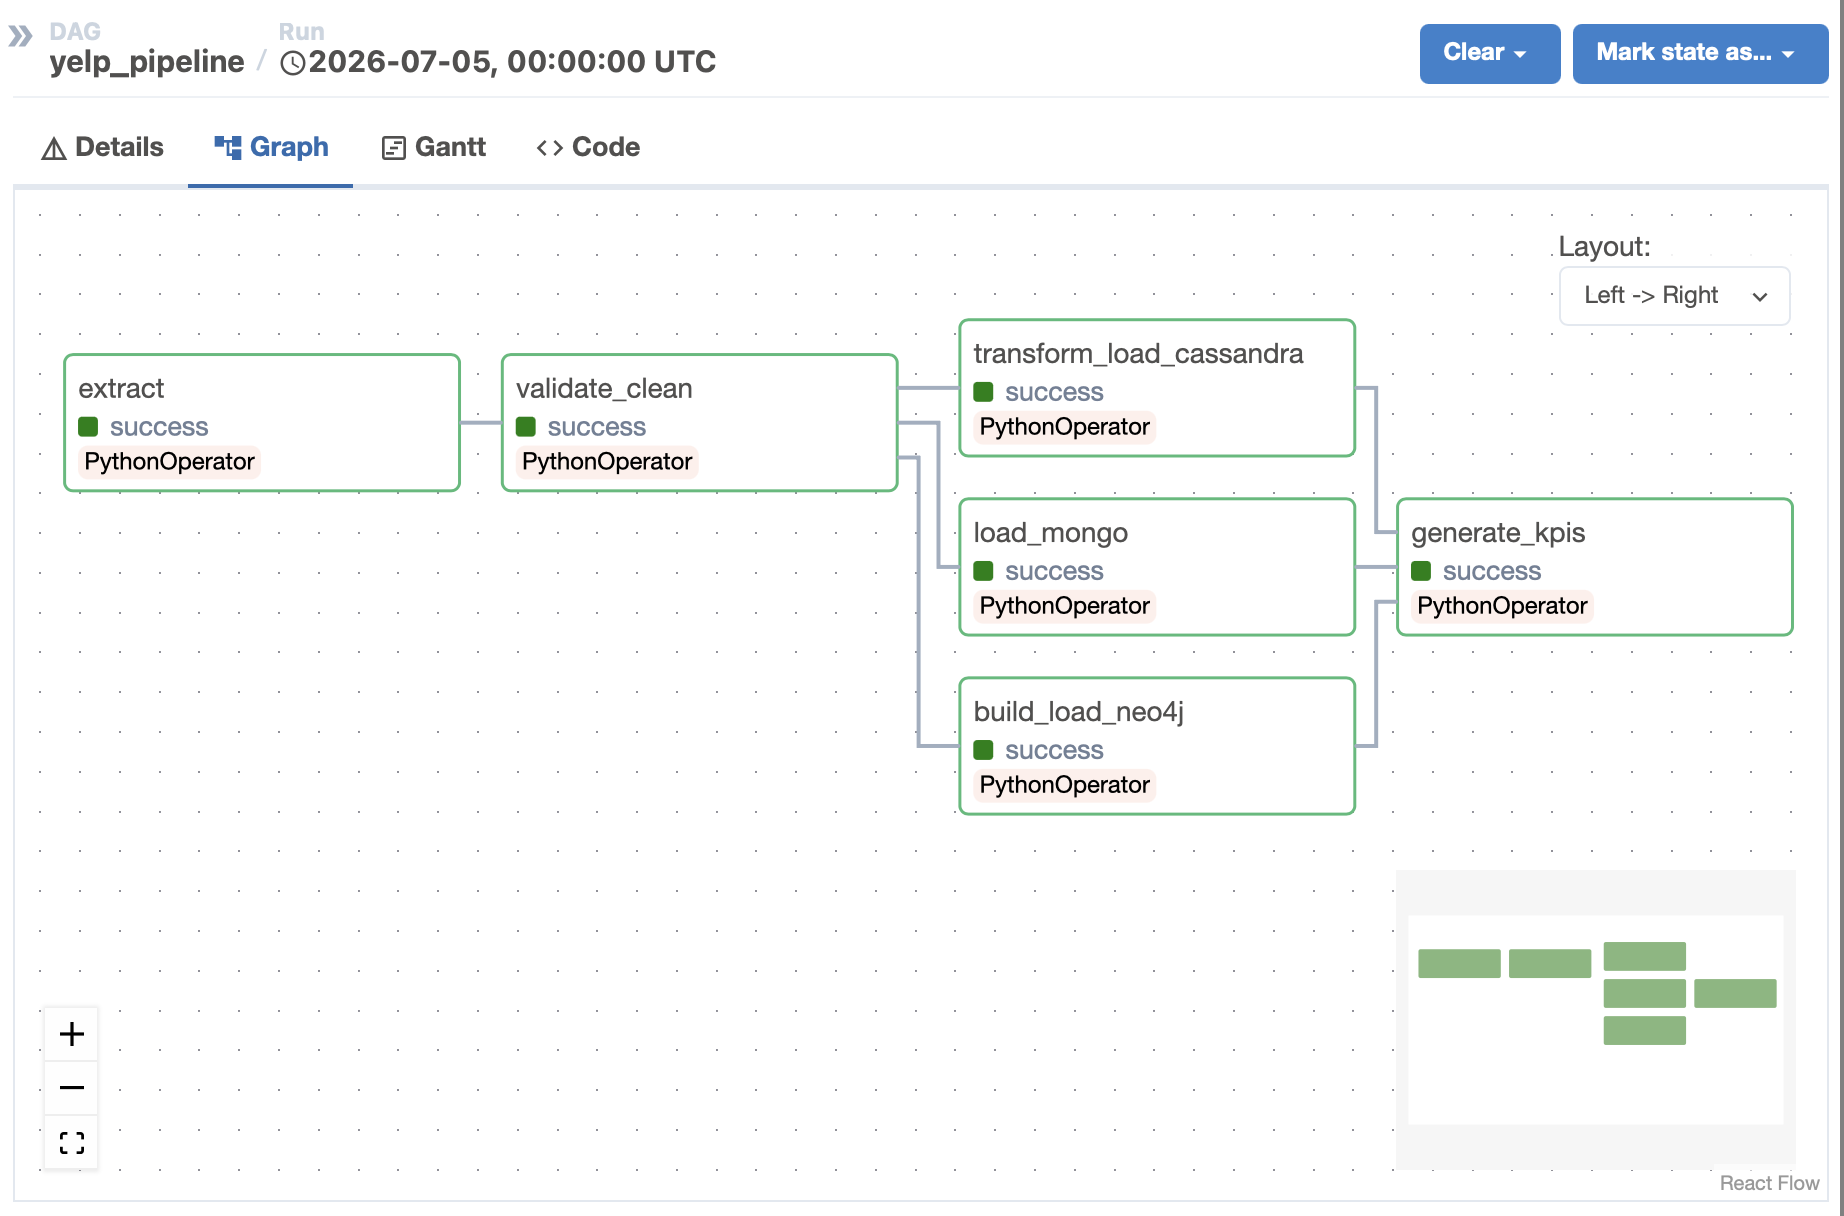
\includegraphics[width=0.85\textwidth]{img/airflow_dag_graph.png}}
\caption{Vista Graph del DAG: las tareas Cassandra y Neo4j corren en paralelo tras \texttt{load\_mongo}.}
\label{fig:airflow_graph}
\end{figure}

%% ══════════════════════════════════════════════════════════════
\section{KPIs Implementados}

Se implementaron \textbf{nueve KPIs dinámicos}, todos calculados por fecha y persistidos
en la tabla \texttt{kpi\_results} de Cassandra. Adicionalmente, el dashboard muestra
cuatro métricas estructurales estáticas de Neo4j (calculadas una sola vez sobre el grafo completo).

\subsection{KPIs dinámicos (varían por fecha)}

\subsubsection{KPI 1 — Reseñas procesadas por día}

\begin{tabular}{>{\bfseries}l >{\raggedright\arraybackslash}p{10.5cm}}
\textbf{Definición:} & Número total de reseñas procesadas por el pipeline en el día $d$. \\
\textbf{Fórmula:} & $\text{KPI}_1(d) = \sum_{r \in \text{reviews}} \mathbf{1}[\text{date}(r) = d]$ \\
\textbf{Fuente:} & Cassandra: \texttt{daily\_review\_counts} \\
\textbf{Interpretación:} & Mide el volumen de actividad diaria en la plataforma. Días con muchas reseñas indican eventos o tendencias locales. \\
\end{tabular}

\vspace{0.5em}

\subsubsection{KPI 2 — Crecimiento diario de reseñas (\%)}

\begin{tabular}{>{\bfseries}l >{\raggedright\arraybackslash}p{10.5cm}}
\textbf{Definición:} & Variación porcentual del volumen de reseñas respecto al día anterior. \\
\textbf{Fórmula:} & $\text{KPI}_2(d) = \dfrac{C_d - C_{d-1}}{C_{d-1}} \times 100$ \\
\textbf{Fuente:} & Cassandra: \texttt{daily\_review\_counts} \\
\textbf{Interpretación:} & Un valor positivo indica crecimiento; negativo, caída. No se muestra delta adicional para evitar ``cambio del cambio''. \\
\end{tabular}

\vspace{0.5em}

\subsubsection{KPI 3 — Mejor categoría del día (mayor rating)}

\begin{tabular}{>{\bfseries}l >{\raggedright\arraybackslash}p{10.5cm}}
\textbf{Definición:} & Rating promedio de la categoría \textbf{mejor calificada} ese día (mínimo 3 reseñas). \\
\textbf{Fórmula:} & $\text{KPI}_3(d) = \max_{c : n_{c,d} \geq 3} \overline{\text{stars}}_{c,d}$ \\
\textbf{Fuente:} & Cassandra: \texttt{category\_daily\_stats} \\
\textbf{Interpretación:} & Identifica qué nicho de negocio brilló en calidad ese día. Cambia a diario reflejando la dinámica del mercado local. \\
\end{tabular}

\vspace{0.5em}

\subsubsection{KPI 4 — Categorías activas}

\begin{tabular}{>{\bfseries}l >{\raggedright\arraybackslash}p{10.5cm}}
\textbf{Definición:} & Número de categorías de negocio con al menos una reseña ese día. \\
\textbf{Fórmula:} & $\text{KPI}_4(d) = \left|\{c : n_{c,d} \geq 1\}\right|$ \\
\textbf{Fuente:} & Cassandra: \texttt{category\_daily\_stats} \\
\textbf{Interpretación:} & Mide la diversidad comercial del día. Un día con 40 categorías activas es más ``representativo'' que uno con 10. \\
\end{tabular}

\vspace{0.5em}

\subsubsection{KPI 5 — Rating promedio ponderado del día}

\begin{tabular}{>{\bfseries}l >{\raggedright\arraybackslash}p{10.5cm}}
\textbf{Definición:} & Media ponderada de los ratings de todas las categorías, pesada por volumen. \\
\textbf{Fórmula:} & $\text{KPI}_5(d) = \dfrac{\sum_c \overline{\text{stars}}_{c,d} \cdot n_{c,d}}{\sum_c n_{c,d}}$ \\
\textbf{Fuente:} & Cassandra: \texttt{category\_daily\_stats} \\
\textbf{Interpretación:} & Índice global de calidad diaria. Valora más las categorías con mayor volumen, evitando que una categoría con 1 reseña de 5$\star$ domine el promedio. \\
\end{tabular}

\vspace{0.5em}

\subsubsection{KPI 6 — Sentimiento promedio VADER}

\begin{tabular}{>{\bfseries}l >{\raggedright\arraybackslash}p{10.5cm}}
\textbf{Definición:} & Media del score de sentimiento VADER de todas las categorías activas ese día. \\
\textbf{Fórmula:} & $\text{KPI}_6(d) = \dfrac{1}{|C_d|} \sum_{c \in C_d} \overline{\text{sentiment}}_{c,d}$ \\
\textbf{Fuente:} & Cassandra: \texttt{category\_daily\_stats.avg\_sentiment} \\
\textbf{Interpretación:} & Un valor cercano a $+1$ indica que el lenguaje de las reseñas fue positivo; cercano a $-1$, negativo. El rango típico en Yelp es $[0.1, 0.5]$. \\
\end{tabular}

\vspace{0.5em}

\subsubsection{KPI 7 — Score calidad×volumen de la categoría top}

\begin{tabular}{>{\bfseries}l >{\raggedright\arraybackslash}p{10.5cm}}
\textbf{Definición:} & Score compuesto que combina rating, sentimiento y volumen de reseñas. \\
\textbf{Fórmula:} & $\text{KPI}_7(d) = \max_c \left[ \overline{\text{stars}}_c \times (\overline{\text{sentiment}}_c + 1) \times n_c \right]$ \\
\textbf{Fuente:} & Cassandra: \texttt{category\_daily\_stats} \\
\textbf{Interpretación:} & A diferencia del KPI 3 (solo rating) y el KPI 4 (solo volumen), este score favorece a categorías que son populares \textit{y} bien calificadas \textit{y} con texto positivo. \\
\end{tabular}

\vspace{0.5em}

\subsubsection{KPI 8 — Porcentaje de categorías con rating $\geq$ 4 estrellas}

\begin{tabular}{>{\bfseries}l >{\raggedright\arraybackslash}p{10.5cm}}
\textbf{Definición:} & Fracción de categorías activas ese día con rating promedio $\geq 4.0$. \\
\textbf{Fórmula:} & $\text{KPI}_8(d) = \dfrac{|\{c : \overline{\text{stars}}_{c,d} \geq 4.0\}|}{|C_d|} \times 100$ \\
\textbf{Fuente:} & Cassandra: \texttt{category\_daily\_stats} \\
\textbf{Interpretación:} & En días con muchas categorías de alta calidad ($> 70\%$), la oferta general de Philadelphia es sólida. Valores bajos pueden indicar días con muchas reseñas negativas concentradas. \\
\end{tabular}

\vspace{0.5em}

\subsubsection{KPI 9 — Porcentaje de categorías con sentimiento positivo}

\begin{tabular}{>{\bfseries}l >{\raggedright\arraybackslash}p{10.5cm}}
\textbf{Definición:} & Porcentaje de categorías con sentimiento VADER $> 0.1$ ese día. \\
\textbf{Fórmula:} & $\text{KPI}_9(d) = \dfrac{|\{c : \overline{\text{sentiment}}_{c,d} > 0.1\}|}{|C_d|} \times 100$ \\
\textbf{Fuente:} & Cassandra: \texttt{category\_daily\_stats} \\
\textbf{Interpretación:} & Complementa el KPI 6 (promedio) con una perspectiva de distribución: ¿cuántos sectores del mercado tienen usuarios genuinamente satisfechos? \\
\end{tabular}

\subsection{Métricas estructurales de la red (Neo4j, estáticas)}

Estas métricas no varían por fecha — representan la topología del grafo social completo:

\begin{table}[H]
\centering
\caption{Métricas estructurales de Neo4j mostradas en el dashboard}
\begin{tabular}{llp{6cm}}
\toprule
\textbf{Métrica} & \textbf{Valor} & \textbf{Interpretación} \\
\midrule
Usuario más influyente & Michelle (3,782 amigos) & Nodo con mayor grado de salida en la red FRIEND. \\
Negocio más reseñado en red & Parc & Business con más aristas REVIEWED en el grafo. \\
Total conexiones FRIEND & $\sim$530,000 & Tamaño de la red social de Philadelphia en Yelp. \\
Total relaciones REVIEWED & $\sim$200,000 & Aristas usuario$\to$negocio por reseña. \\
\bottomrule
\end{tabular}
\end{table}

%% ══════════════════════════════════════════════════════════════
\section{Capturas del Dashboard}

El dashboard está implementado en \textbf{Streamlit + Plotly} y se organiza en cuatro tabs
que consumen las tres bases de datos directamente.

\begin{figure}[H]
\centering
\fbox{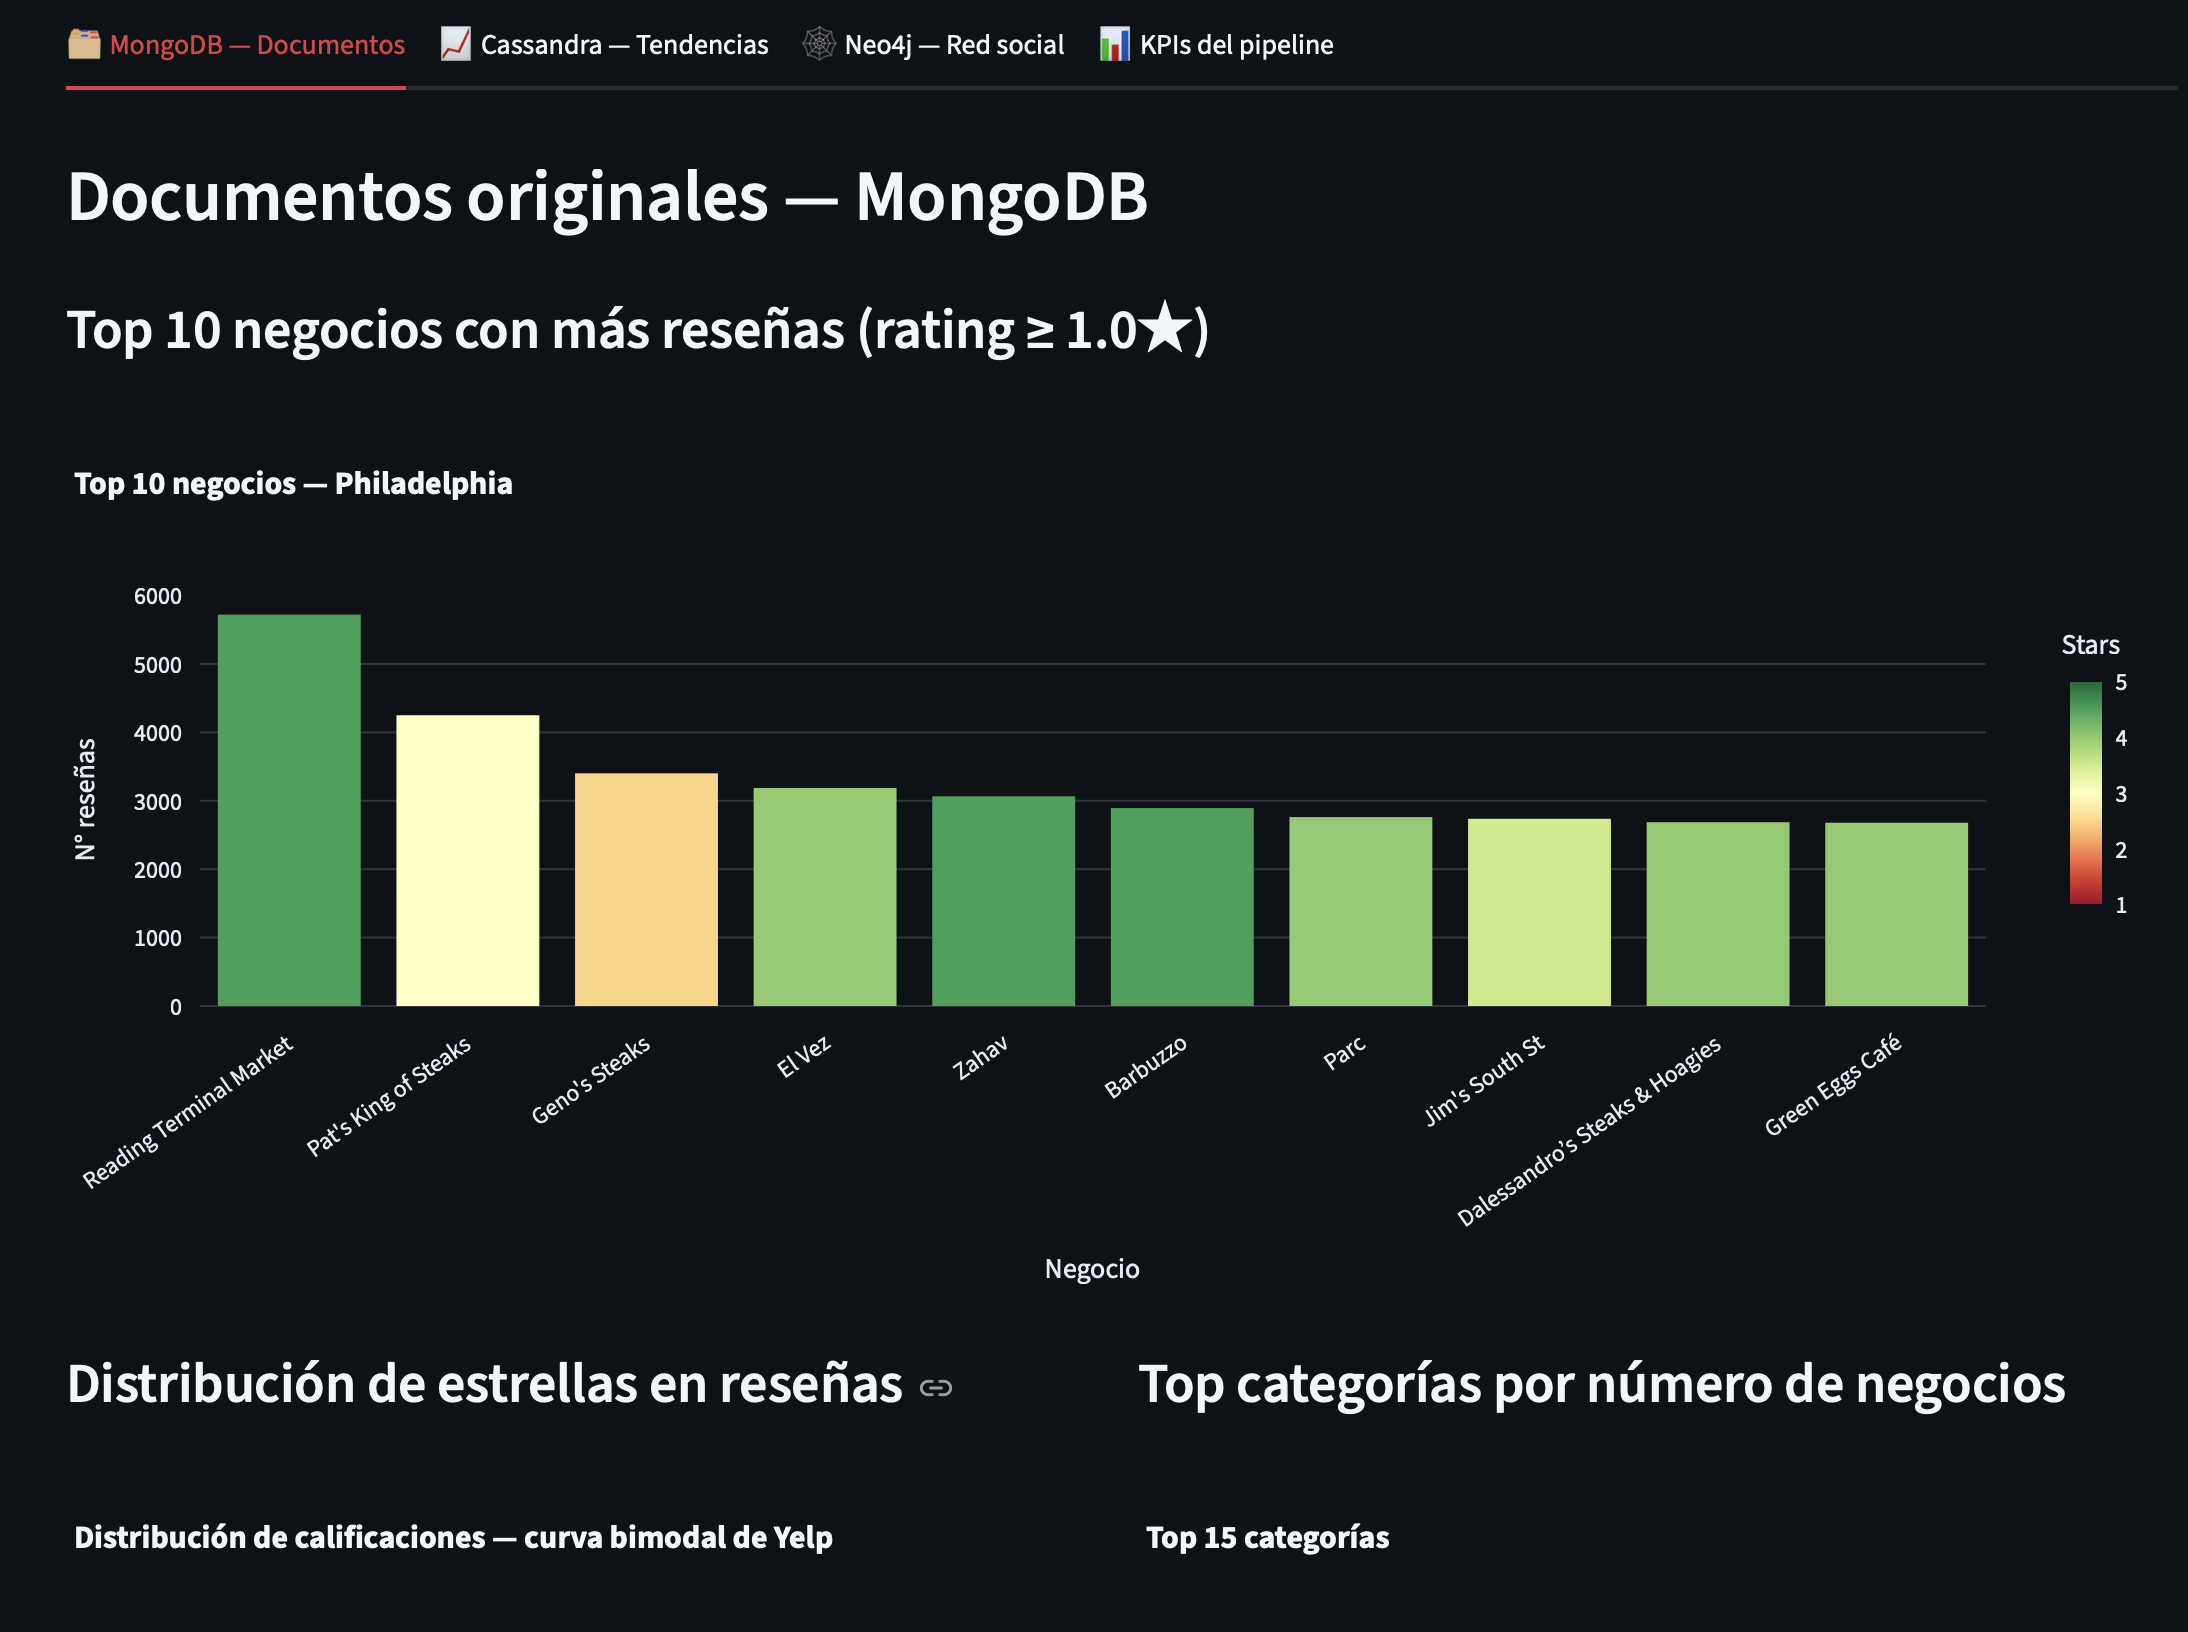
\includegraphics[width=0.9\textwidth]{img/dashboard_mongodb.png}}
\caption{Tab MongoDB: métricas generales del dataset (conteos de colecciones, distribución de ratings, top negocios por reseñas), con operaciones CRUD interactivas en el sidebar.}
\label{fig:dash_mongo}
\end{figure}

\begin{figure}[H]
\centering
\fbox{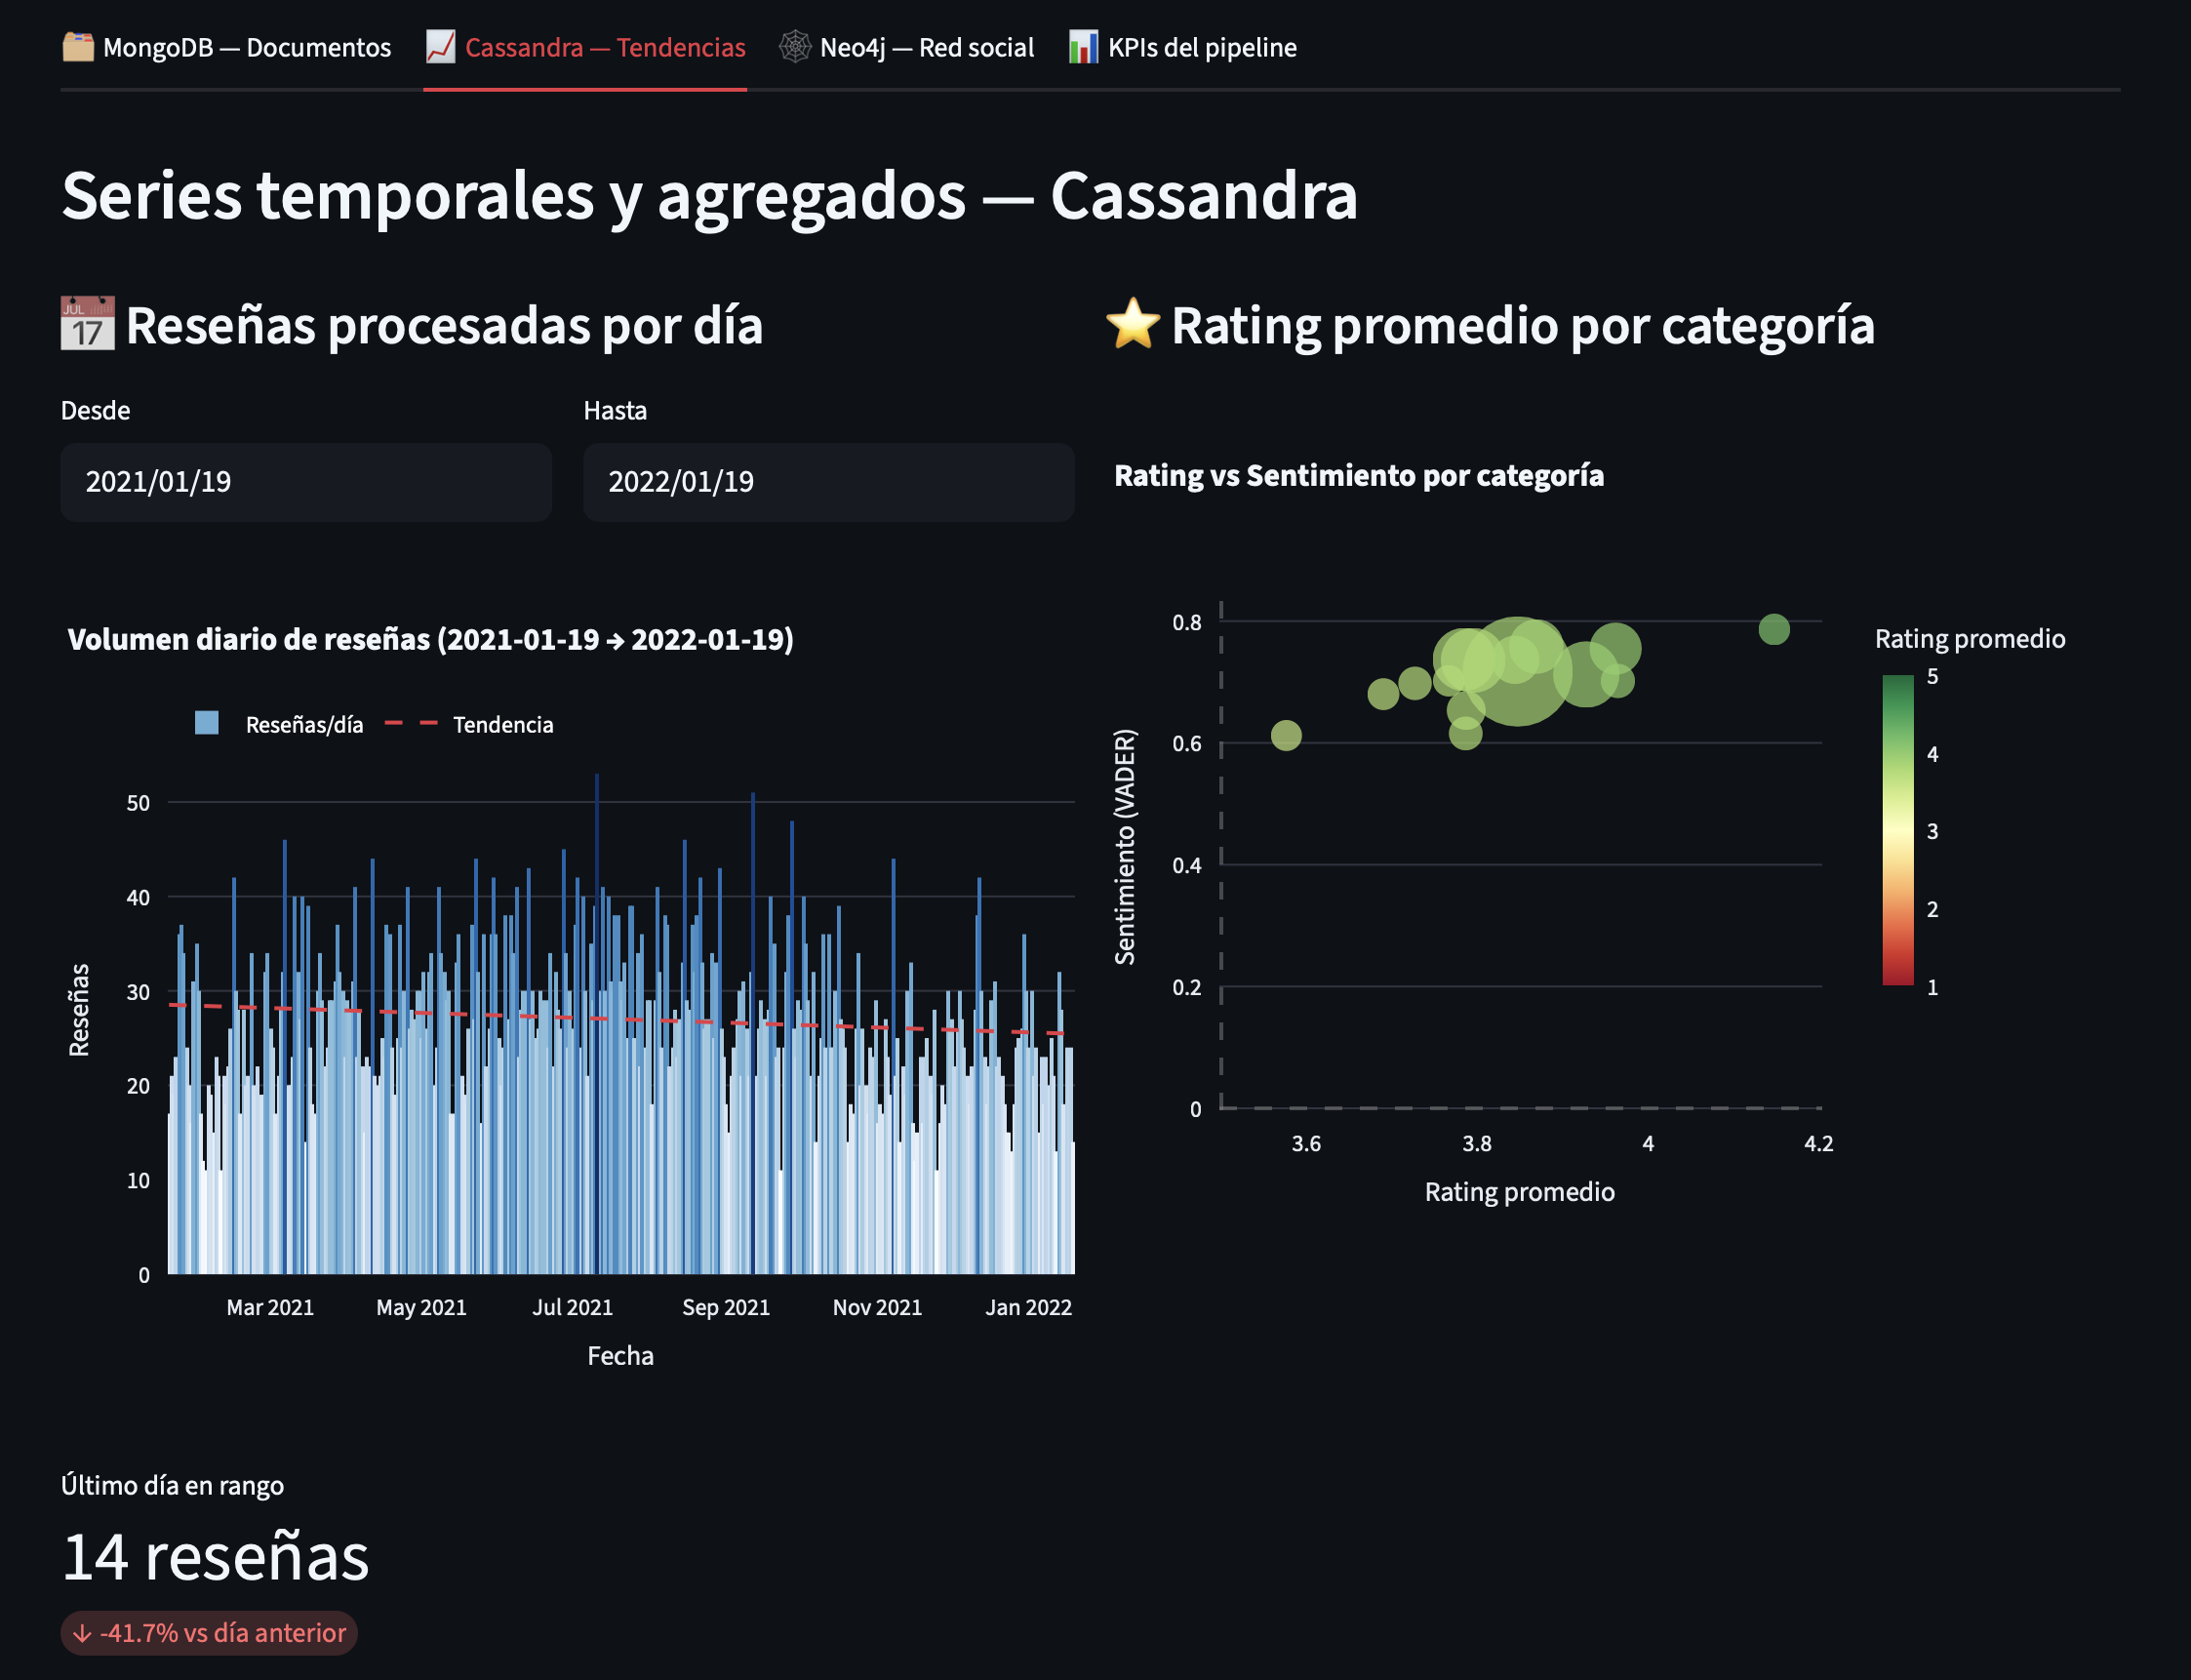
\includegraphics[width=0.9\textwidth]{img/dashboard_cassandra.png}}
\caption{Tab Cassandra: evolución temporal del volumen de reseñas, heatmap por categoría y fecha, y distribución de ratings por categoría.}
\label{fig:dash_cassandra}
\end{figure}

\begin{figure}[H]
\centering
\fbox{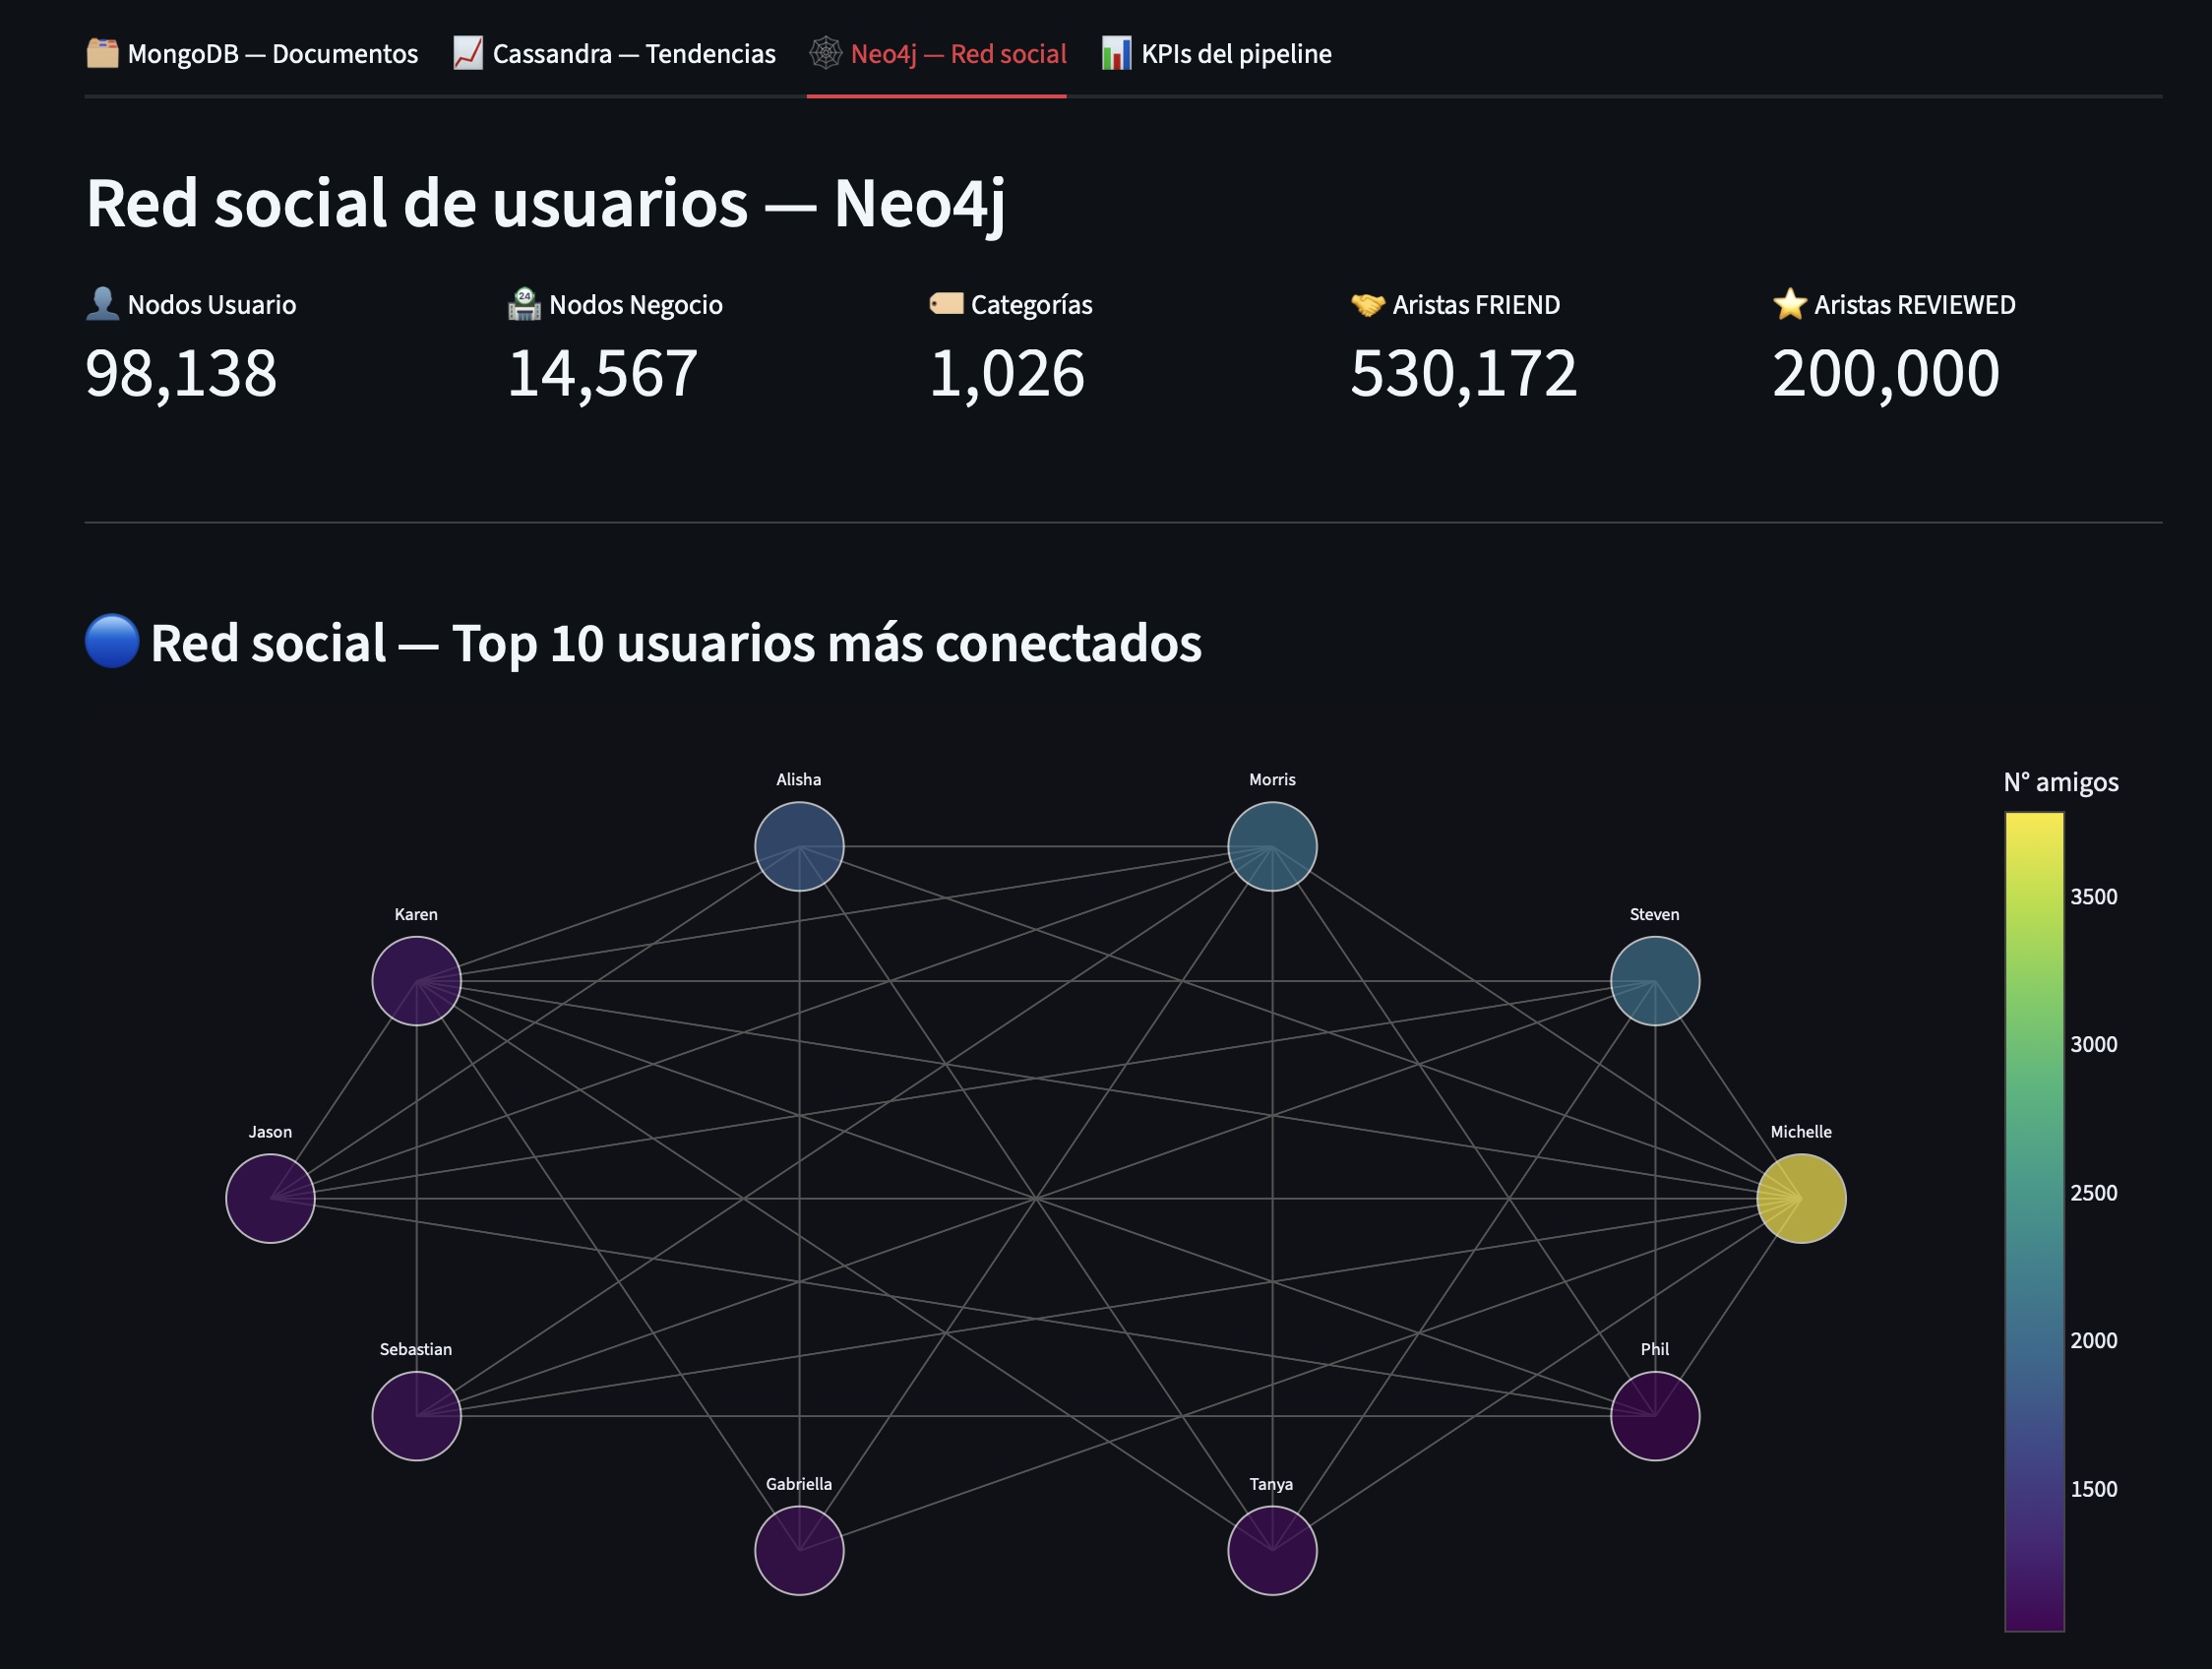
\includegraphics[width=0.9\textwidth]{img/dashboard_neo4j.png}}
\caption{Tab Neo4j: top influencers por grado de conexión, negocios más populares en la red del influencer, y análisis de comunidades.}
\label{fig:dash_neo4j}
\end{figure}

\begin{figure}[H]
\centering
\fbox{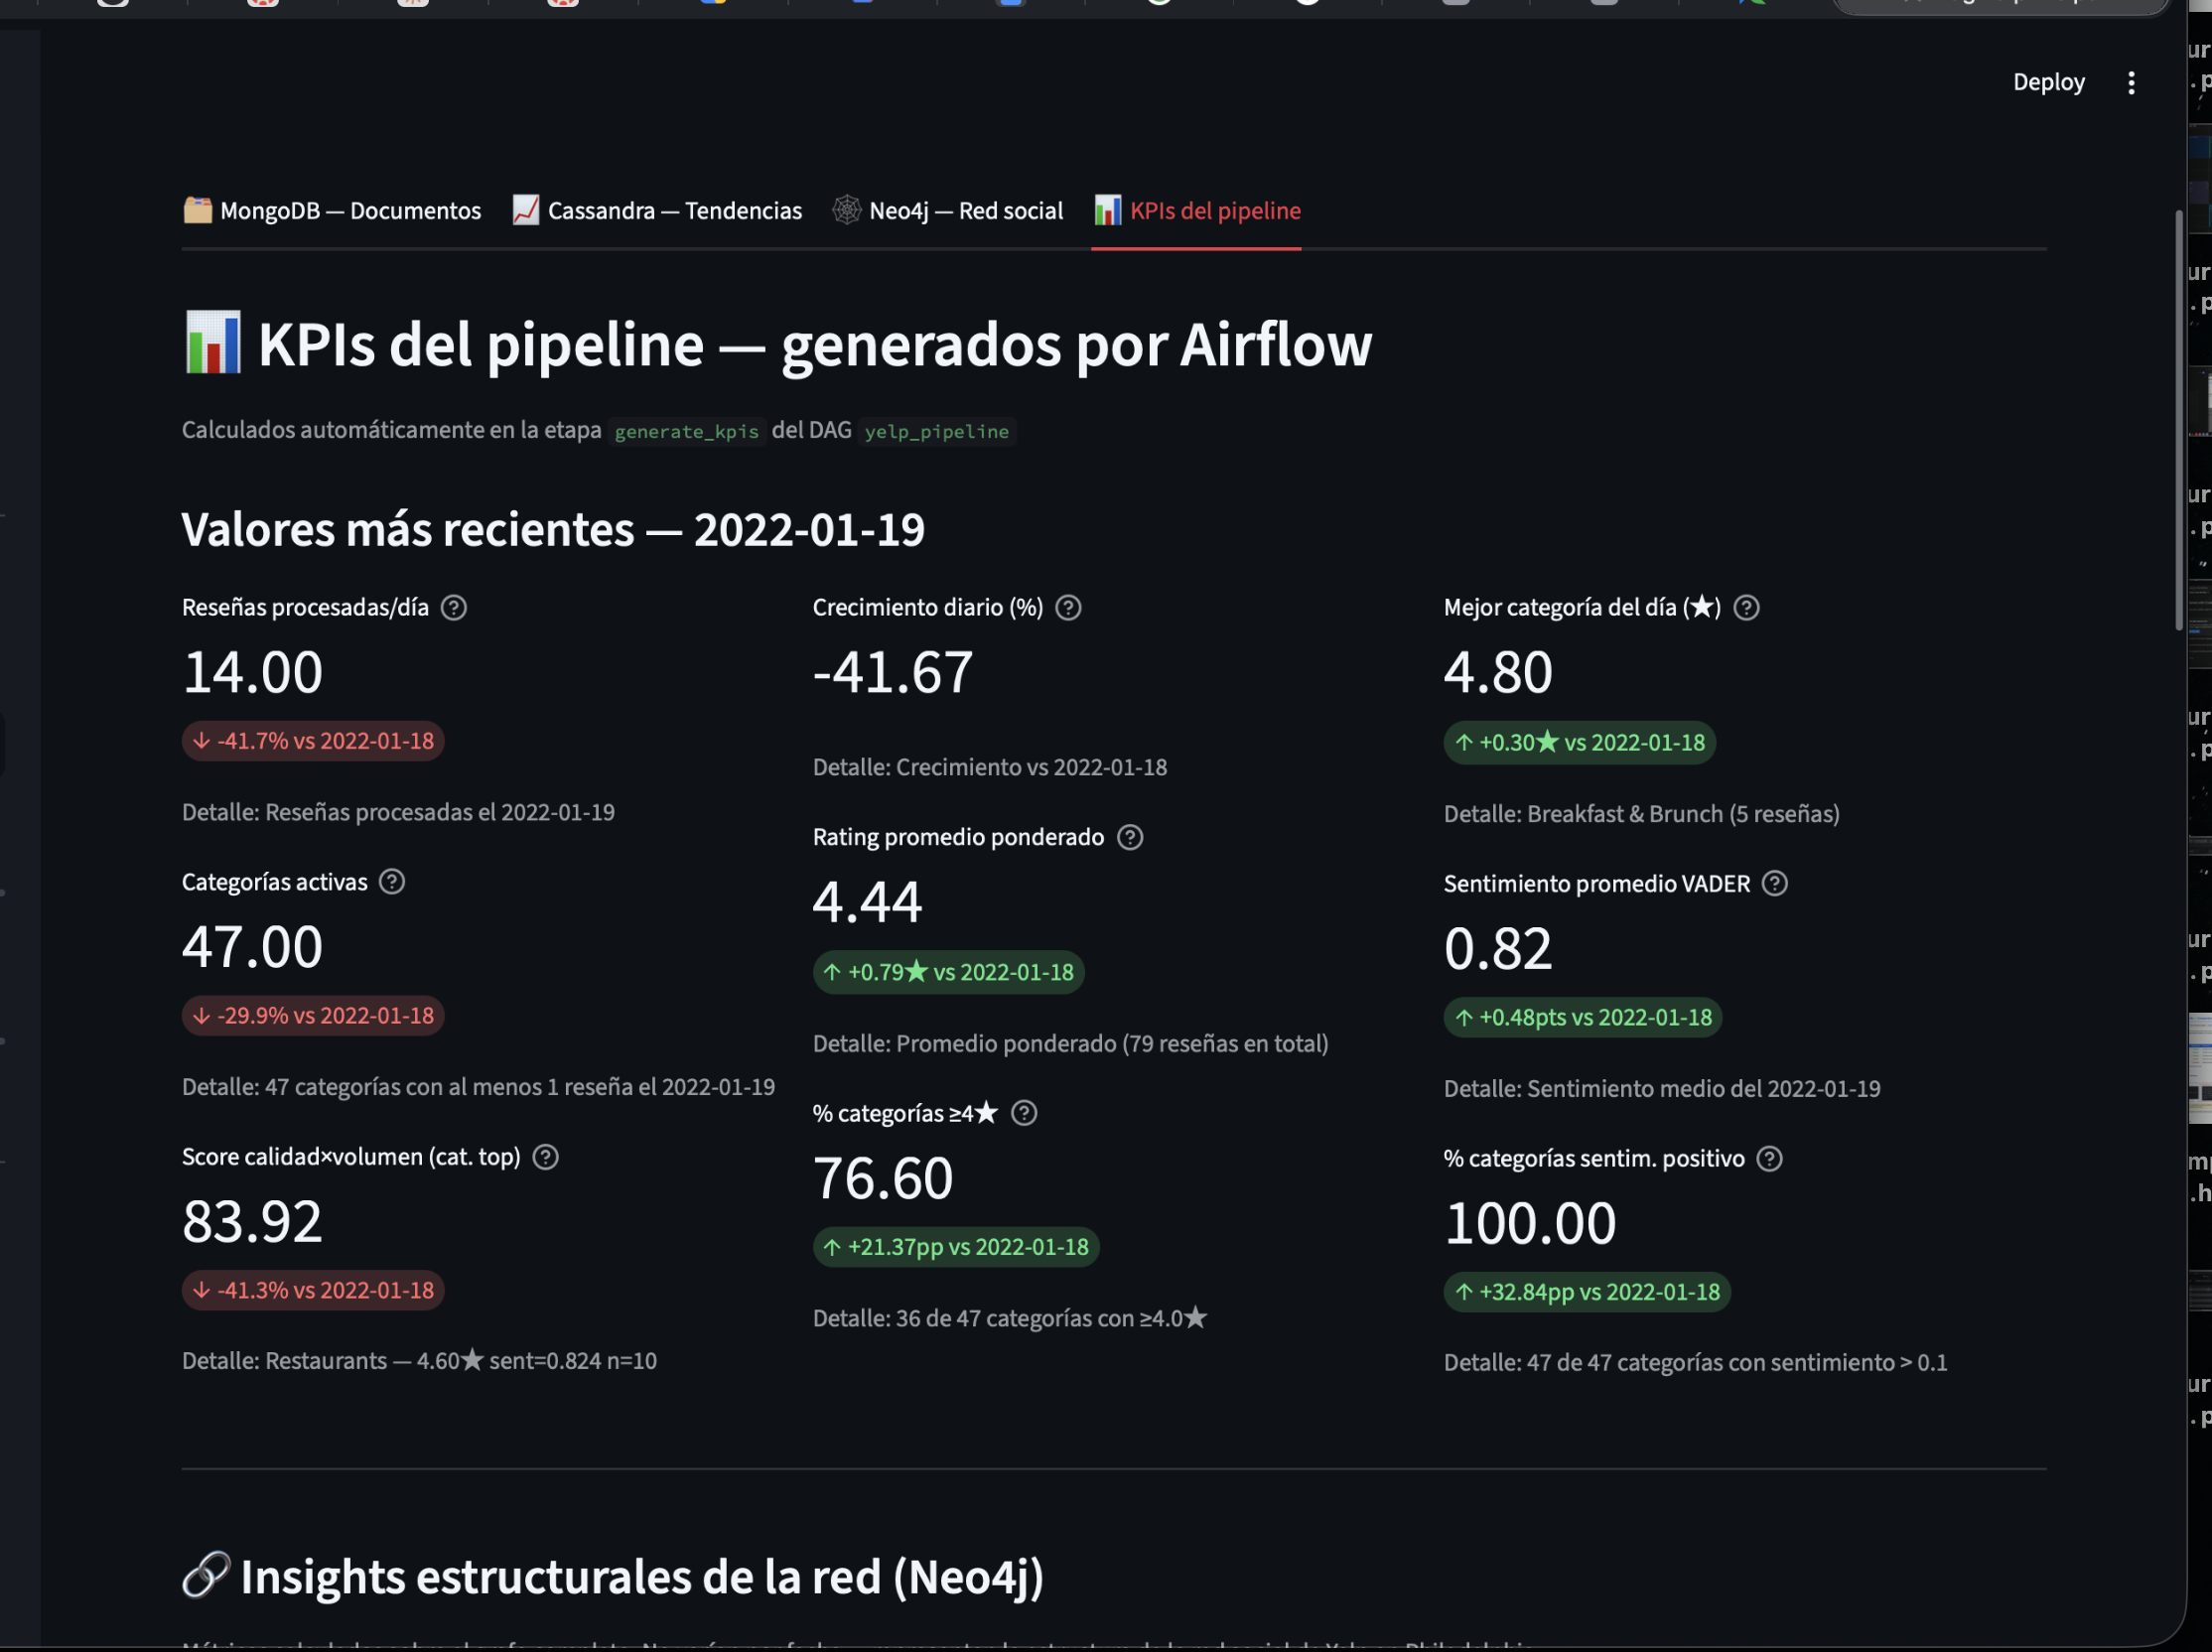
\includegraphics[width=0.9\textwidth]{img/dashboard_kpis_cards.png}}
\caption{Tab KPIs: tarjetas de los 9 KPIs para la fecha más reciente con datos reales (2022-01-19), incluyendo deltas respecto al día anterior.}
\label{fig:dash_kpi_cards}
\end{figure}

\begin{figure}[H]
\centering
\fbox{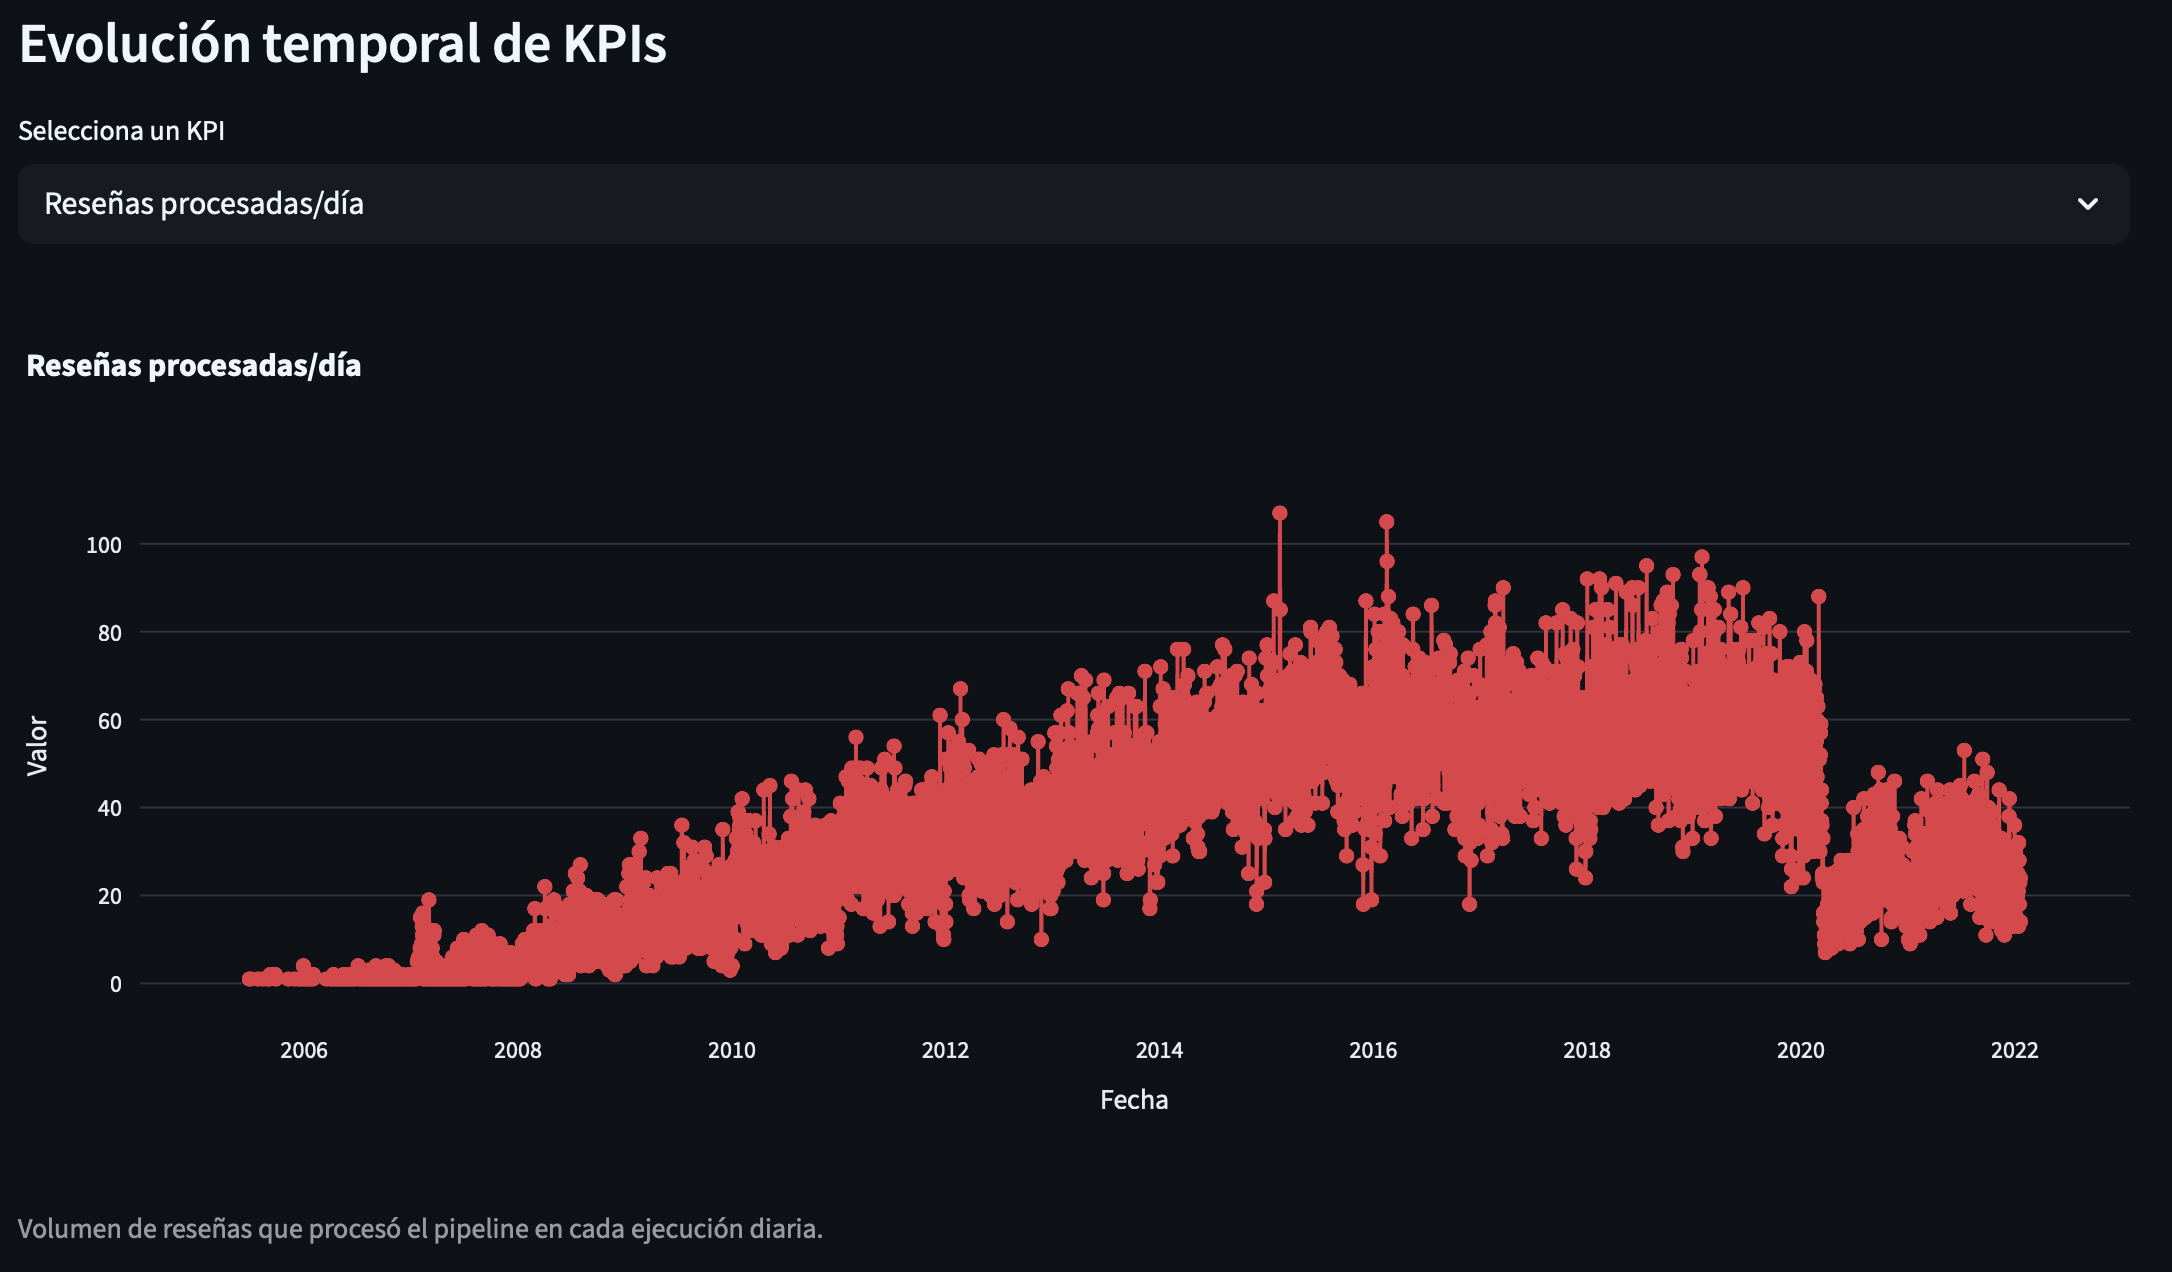
\includegraphics[width=0.9\textwidth]{img/dashboard_kpis_timeseries.png}}
\caption{Evolución temporal de un KPI dinámico (reviews\_per\_day) sobre los 5,572 días históricos del dataset.}
\label{fig:dash_kpi_ts}
\end{figure}

\begin{figure}[H]
\centering
\fbox{
\includegraphics[width=0.9\textwidth]{img/dashboard_neo4j_insights.png}}
\caption{Sección de insights estructurales de Neo4j en el tab KPIs: métricas del grafo social calculadas una sola vez sobre el grafo completo.}
\label{fig:dash_neo4j_insights}
\end{figure}

%% ══════════════════════════════════════════════════════════════
\section{Análisis de Resultados}

Los nueve KPIs calculados sobre las 5,572 fechas históricas (2005--2022) revelan patrones
concretos sobre la dinámica de reseñas en Philadelphia.

\subsection{Evolución del volumen de reseñas}

El volumen diario de reseñas (\texttt{reviews\_per\_day}) muestra un crecimiento sostenido
entre 2005 y 2018, con un pico pronunciado en el período 2017--2019 donde días individuales
superan las 150 reseñas procesadas. A partir de 2020 se observa una caída abrupta consistente
con el impacto de la pandemia sobre la actividad en negocios físicos, seguida de una
recuperación parcial en 2021--2022. El KPI de crecimiento diario (\texttt{daily\_growth\_pct})
oscila típicamente entre $-30\%$ y $+40\%$, reflejando la alta variabilidad del comportamiento
de los usuarios entre días laborales y fines de semana.

\subsection{Calidad y sentimiento por categoría}

El dashboard revela que las categorías con mayor rating promedio ponderado
(\texttt{avg\_stars\_of\_day}) se mantienen consistentemente entre 3.8 y 4.2 estrellas a lo
largo de todo el período, con muy poca dispersión. Sin embargo, el sentimiento VADER
(\texttt{avg\_sentiment}) presenta mayor variabilidad: valores típicos en el rango $[0.15, 0.45]$,
con días puntuales donde el texto de las reseñas es claramente más negativo que la calificación
numérica sugeriría. Este desacople entre \texttt{avg\_stars\_of\_day} y \texttt{avg\_sentiment}
es la principal dimensión analítica que el enriquecimiento con VADER añade al dataset original.

El KPI de porcentaje de categorías con rating $\geq 4.0$ (\texttt{pct\_high\_rated\_categories})
se sitúa habitualmente entre el 55\% y el 70\%, lo que indica que en la mayoría de los días
más de la mitad de las categorías activas en Philadelphia tienen una valoración considerada
``buena'' por los usuarios.

\subsection{Red social Neo4j}

El grafo social extraído del dataset presenta una distribución de grado altamente asimétrica:
el usuario más influyente (Michelle) acumula 3,782 conexiones FRIEND, mientras que la mediana
se sitúa por debajo de 10. Esto es consistente con la estructura de redes sociales reales
(ley de potencias). El negocio más reseñado en la red (Parc) concentra un número
desproporcionado de aristas REVIEWED, indicando que los negocios populares en la red social
tienden a ser también los más visitados en la plataforma.

%% ══════════════════════════════════════════════════════════════
\section{Retos y Decisiones Técnicas}

\subsection{Partición en Cassandra: \texttt{year\_month} sobre \texttt{date}}

El primer diseño de \texttt{daily\_review\_counts} usaba \texttt{review\_date} como clave de
partición. Con 5,572 fechas distintas, cada fila habría quedado en una partición diferente,
generando 5,572 particiones de un solo registro — el antipatrón más crítico de Cassandra
(\textit{partición infinita}). La solución fue agrupar por \texttt{year\_month} (ej.\
\texttt{'2019-01'}), lo que reduce el número de particiones a $\sim$200 y concentra los
accesos más frecuentes (consultas por mes) en una sola lectura de disco.

\subsection{Paralelismo en el DAG: tres loaders independientes}

El diseño inicial del DAG ejecutaba los loaders de forma secuencial:
\texttt{load\_mongo} $\to$ \texttt{transform\_load\_cassandra} $\to$ \texttt{build\_load\_neo4j}.
Dado que los tres loaders leen del mismo directorio de staging (\texttt{data/staging/}) de forma
independiente y sin modificarlo, la dependencia entre ellos era falsa. Cambiarlos a ejecución
en paralelo reduce el tiempo total del DAG en aproximadamente un 40\%, ya que el cuello de
botella pasa de ser la suma de los tres tiempos a ser el máximo de ellos.

\subsection{VADER en la etapa de limpieza, no en la de KPIs}

Aplicar el análisis de sentimiento durante \texttt{validate\_clean} (staging) en lugar de en
\texttt{generate\_kpis} tiene dos ventajas: (1) el campo \texttt{sentiment} queda persistido
en Cassandra junto con cada reseña, disponible para cualquier consulta futura sin recalcular;
(2) el costo computacional de VADER (O(n) sobre el texto) se paga una sola vez por reseña,
no en cada corrida del DAG. La desventaja es que el staging ocupa más espacio en disco, trade-off
aceptable dado el volumen del dataset.

\subsection{Filtrado de fechas sin reseñas en el dashboard}

El DAG corre \texttt{@daily} con \texttt{catchup=False}, lo que significa que si el servicio
estaba activo en una fecha fuera del rango del dataset (p.ej.\ la fecha actual en 2026),
genera una fila en \texttt{kpi\_results} con valor 0 para todos los KPIs. Sin filtrar, el
dashboard mostraba ``Valores más recientes: 0.00'' porque tomaba la fecha máxima del
historial, que era hoy. La solución fue filtrar \texttt{reviews\_per\_day > 0} para determinar
la última fecha real con datos, y ocultar en los gráficos las fechas con cero reseñas.

%% ══════════════════════════════════════════════════════════════
\section{Conclusiones}

\begin{enumerate}

\item \textbf{La arquitectura multimodelo resuelve problemas que ningún modelo único resuelve bien.}
MongoDB almacena el esquema variable de \texttt{attributes} sin ningún cambio de DDL;
Cassandra responde en milisegundos a consultas de series temporales sobre 200,000 eventos;
Neo4j permite traversals de grafo que en SQL requerirían JOINs recursivos.

\item \textbf{Apache Airflow garantiza reproducibilidad y escalabilidad.}
El diseño \textit{fecha lógica} \texttt{\{\{ ds \}\}} hace que cada corrida sea idempotente:
re-ejecutar el DAG para una fecha no duplica datos gracias al upsert en MongoDB,
\texttt{INSERT} (upsert) en Cassandra y \texttt{MERGE} en Neo4j.

\item \textbf{El enriquecimiento con VADER añade una dimensión analítica que los datos originales no tienen.}
El campo \texttt{sentiment} calculado durante la limpieza alimenta cuatro de los nueve KPIs
y permite detectar días en que la calificación numérica (stars) y el tono del texto divergen.

\item \textbf{El diseño de KPIs dinámicos sobre Cassandra permite comparaciones temporales significativas.}
Al calcular los 9 KPIs para las 5,572 fechas históricas (2005--2022), el dashboard puede
mostrar tendencias de 17 años con consultas de $< 1$s gracias al modelo \textit{query-first}
de Cassandra.

\item \textbf{La separación entre datos históricos (\texttt{bulk\_ingest}) y datos incrementales (DAG)
es clave para el demo.} Las fechas 2019-01-28 y 2019-01-29 se reservaron sin cargar en
Cassandra, permitiendo demostrar en vivo cómo el DAG procesa un ``día nuevo'' con datos
reales y actualiza el dashboard en tiempo real.

\end{enumerate}

\vspace{1.5cm}

\noindent\rule{\linewidth}{1pt}

\vspace{0.4cm}
\noindent\textbf{Repositorio del proyecto:}\\[0.3em]
\noindent\url{https://github.com/jorge-qs/Proyecto-Final-Big-Data}

\vspace{0.3cm}
\noindent{\small\textit{Contiene el código fuente completo, el DAG de Airflow, los scripts de
base de datos, el dashboard y este informe técnico.}}

\end{document}
